% =====================================================================
% Project: Software Engineering (DLMCSPSE01)
% Portfolio Part 3 -- Finalisation Phase: complete project documentation
% Compile: pdflatex <file>.tex  (run TWICE for contents and references)
% Requires: logo.png and the folder screenshots/ next to this file.
% Screenshots not yet present are shown as labelled placeholder boxes.
%
% Screenshots used:
%   screenshots/kanban_board.jpg                  Figure 1
%   screenshots/report_M05.jpg                    Figure 4
%   screenshots/start_page.jpg, test_run.jpg, render_live.jpg and
%   screenshots/appendix/*.jpg                    Appendix A
\documentclass[a4paper,11pt]{article}

\usepackage[top=2cm, bottom=2cm, left=2cm, right=2cm]{geometry}
\usepackage[utf8]{inputenc}
\usepackage[T1]{fontenc}
\usepackage{helvet}
\renewcommand{\familydefault}{\sfdefault}
\usepackage{setspace}
\onehalfspacing
\usepackage{parskip}
\setlength{\parskip}{6pt}
\setlength{\parindent}{0pt}
\setlength{\emergencystretch}{2em}
\usepackage{graphicx}
\usepackage{tikz}
\usetikzlibrary{shapes.geometric, arrows.meta, positioning, calc}
\usepackage{booktabs}
\usepackage{tabularx}
\usepackage{hyperref}
\hypersetup{colorlinks=true, linkcolor=black, citecolor=blue, urlcolor=blue}
\usepackage[round]{natbib}
\usepackage{fancyhdr}
\usepackage{caption}
\usepackage{subcaption}
\captionsetup[subfigure]{list=false}
\usepackage{enumitem}
\usepackage{xcolor}
% colortbl, NOT xcolor's [table] option -- TikZ already loads xcolor.
\usepackage{colortbl}
\usepackage{float}
\usepackage{array}
\usepackage{xurl}

\pagestyle{fancy}
\fancyhf{}
\fancyfoot[C]{\thepage}
\renewcommand{\headrulewidth}{0pt}

\usepackage{titlesec}
\titleformat{\section}{\normalfont\fontsize{12}{14}\bfseries}{\thesection}{1em}{}
\titleformat{\subsection}{\normalfont\fontsize{11}{13}\bfseries}{\thesubsection}{1em}{}
\titlespacing*{\section}{0pt}{12pt}{4pt}
\titlespacing*{\subsection}{0pt}{9pt}{3pt}
\setcounter{tocdepth}{2}

% Screenshot with automatic placeholder: #1 file, #2 width, #3 what it must show
\newcommand{\screenshot}[3]{%
  \IfFileExists{#1}{%
    \fbox{\includegraphics[width=#2]{#1}}%
  }{%
    \fbox{\parbox[c][5cm][c]{#2}{\centering\small\color{red!70!black}
      \textbf{Screenshot to be inserted}\\[4pt]
      \texttt{\detokenize{#1}}\\[6pt]
      \color{black!70}#3}}%
  }%
}

% Diagram styles
\tikzset{
  system/.style = {draw, rounded corners=2pt, align=center, fill=blue!12,
                   draw=blue!55, minimum width=3.6cm, minimum height=1.2cm,
                   font=\scriptsize\bfseries, inner sep=4pt},
  actor/.style  = {draw, ellipse, fill=gray!12, align=center, font=\scriptsize, inner sep=3pt},
  ext/.style    = {draw, rounded corners=2pt, align=center, fill=gray!12,
                   font=\scriptsize, minimum height=0.8cm, inner sep=4pt},
  flow/.style   = {-{Latex[length=2mm]}, thick, draw=black!65},
  dep/.style    = {-{Straight Barb[length=2.4mm]}, dashed, draw=black!70},
  node3d/.style = {draw=black!60, fill=gray!8, align=center, font=\scriptsize, inner sep=5pt}
}

% UML component icon; the coordinate given is the icon's right edge.
\newcommand{\compicon}[2]{%
  \begin{scope}[shift={(#1,#2)}, draw=black!55, line width=0.4pt]
    \fill[white] (-0.24,-0.09) rectangle (0,0.09);  \draw (-0.24,-0.09) rectangle (0,0.09);
    \fill[white] (-0.30,0.015) rectangle (-0.18,0.065); \draw (-0.30,0.015) rectangle (-0.18,0.065);
    \fill[white] (-0.30,-0.065) rectangle (-0.18,-0.015); \draw (-0.30,-0.065) rectangle (-0.18,-0.015);
  \end{scope}
}

% Shared table setup
\newcommand{\tablesetup}{\footnotesize\renewcommand{\arraystretch}{1.2}\setlength{\tabcolsep}{4pt}}
\newcolumntype{L}[1]{>{\raggedright\arraybackslash}p{#1}}
\renewcommand{\tabularxcolumn}[1]{>{\raggedright\arraybackslash}p{#1}}

\begin{document}

% =====================================================================
% TITLE PAGE
% =====================================================================
\begin{titlepage}
\thispagestyle{empty}
\noindent
\includegraphics[width=7cm]{logo.png}

\vspace{1.2cm}
\noindent\rule{\textwidth}{0.6pt}
\vspace{0.15cm}
\begin{center}
{\Large\textbf{PortfolioCheck: Design, Development and Evaluation\\of a Web Application for the Automated Verification\\of Formal Coursework Submission Requirements}}
\end{center}
\vspace{0.05cm}
\noindent\rule{\textwidth}{0.6pt}

\vspace{1.5cm}
\begin{center}
{\large\textbf{Course: Project: Software Engineering (DLMCSPSE01)}}
\end{center}
\vspace{1.2cm}
\begin{center}
{\large\textbf{Portfolio Part 3 --- Finalisation Phase}}
\end{center}

\vspace{1.0cm}
\noindent
\begin{tabular}{@{}p{5.5cm} p{7cm}@{}}
\\[0.6cm]
\textbf{Degree Programme:}     & \textbf{Master of Science (M.Sc.)} \\[0.9cm]
\textbf{Name of Author:}       & \textbf{Siva Kondaru} \\[0.9cm]
\textbf{Matriculation Number:} & \textbf{10243569} \\[0.9cm]
\textbf{Name of Tutor:}        & \textbf{Holger Klus} \\[0.9cm]
\textbf{Date:}                 & \textbf{October 2026} \\[0.9cm]
\end{tabular}
\end{titlepage}

% =====================================================================
% FRONT MATTER
% =====================================================================
\pagenumbering{Roman}
\setcounter{page}{2}

\section*{Abstract}
\addcontentsline{toc}{section}{Abstract}

This document is the complete project documentation of \textit{PortfolioCheck},
a web application that verifies a coursework portfolio submission against the
formal requirements of its assignment brief before the student hands it in. It
consolidates the conception and development phases, revised in response to the
tutorial feedback, and adds the implementation, testing and deployment results
of the finalisation phase. A student uploads the zip folder they intend to
submit; the application evaluates it against seven rules derived from the brief
and returns a report in which every problem is paired with the exact correction
required and with the provision of the brief it derives from. The most
distinctive rule compares the submitted code archive with the public GitHub
repository file by file, using the content hashes that git itself uses. The
project was managed with Kanban, with the board moved into GitHub Projects after
the Phase~2 feedback, the architecture is
documented in a UML component and a UML deployment view, and the application
is verified by 73 automated tests and thirteen manual test cases. All thirteen
functional requirements are implemented. The document closes with the remaining
technical debt and the lessons learned.

\textbf{Keywords:} software engineering, requirements engineering, software
architecture, UML, Kanban, software testing, technical debt

\newpage
\tableofcontents
\vspace{0.6cm}
\listoffigures
\vspace{0.3cm}
\listoftables
\newpage

\section*{List of Abbreviations}
\addcontentsline{toc}{section}{List of Abbreviations}
\begin{tabularx}{\textwidth}{@{}l X@{}}
\toprule
\textbf{Abbreviation} & \textbf{Definition} \\
\midrule
API   & Application Programming Interface \\
FR    & Functional Requirement \\
HTTP  & Hypertext Transfer Protocol \\
ISO   & International Organization for Standardization \\
NFR   & Non-Functional Requirement \\
PDF   & Portable Document Format \\
REST  & Representational State Transfer \\
TD    & Technical Debt \\
UML   & Unified Modeling Language \\
WIP   & Work in Progress \\
WP    & Work Package \\
\bottomrule
\end{tabularx}
\newpage

% =====================================================================
% MAIN TEXT
% =====================================================================
\pagenumbering{arabic}
\setcounter{page}{1}

% =====================================================================
\section{Introduction}\label{sec:intro}
% =====================================================================

\subsection{Problem and Objective}\label{sec:problem}

Every portfolio submission in a distance-learning degree programme is governed by
purely formal provisions. The brief of this course alone prescribes a naming
pattern for the main directory, a second pattern for the code archive and a third
for each phase document; four subdirectories whose names must match exactly;
permitted file formats; a size limit of 15\,MB; a links file with the repository
address, the application address and any login data; and the requirement that
the public repository and the submitted code archive be identical. These
provisions exist so that examination offices can process large numbers of
submissions consistently --- the same pressure of scale that drives automation
elsewhere in educational assessment \citep{Paiva2022}.

The provisions are deterministic, verifiable without human judgement and
numerous, and they are checked at the worst possible moment: in the final hours
before a deadline, when the attention available for mechanical detail is at its
lowest \citep{Hermans2021}. Research on automated assessment concentrates on
the \textit{content} of student work, above all the correctness of program code
\citep{Messer2024, Combefis2022}; the formal envelope of a submission has
received almost no attention. Students therefore check it by hand, without any
confirmation of success, and discover errors only when they can no longer be
corrected.

The objective of the project was a web application that accepts the archive a
student intends to submit, evaluates it against the formal requirements, and
returns a report stating for each requirement whether it is met and, if not,
exactly what must be changed. That last element is decisive: feedback that names
the correction is what gives automated assessment its practical value, whereas a
bare verdict merely restates the problem \citep{Combefis2022}.

The document follows the course of the project. Section~\ref{sec:theory}
summarises the theory the project builds on. Chapter~\ref{sec:management}
describes how the project was organised: its profile, the work packages and their
dates, the Kanban workflow and the risks. Chapter~\ref{sec:reqarch} states what
the system must do and how it is built: the requirements, the glossary, two UML
architecture views and the technology stack. Chapter~\ref{sec:impl} reports what
was built and shows that it works: the implementation, the manual and automated
tests, the results and the deployment. Chapter~\ref{sec:reflection} closes with
the technical debt, the lessons learned and a conclusion. This order mirrors the
life cycle of a software product, from planning to evaluation
\citep{Sommerville2020}.

\subsection{Revisions after the Phase 2 Feedback}\label{sec:revisions}

This document revises the Phase~2 document and completes it for the final
submission. Table~\ref{tab:changes} shows how each point of the Phase~2 feedback
was addressed, so that the development of the work remains traceable across the
portfolio phases \citep{Bass2021}.

\begin{table}[!t]
\centering
\caption{Phase 2 feedback and how it was addressed}
\label{tab:changes}
\tablesetup
\begin{tabularx}{\textwidth}{|c|L{5.4cm}|X|}
\hline
\rowcolor{gray!15}
\textbf{No.} & \textbf{Feedback} & \textbf{How it was addressed} \\
\hline\hline
1 & Include specific dates in the project plan & Every work package and milestone has calendar dates (Table~\ref{tab:workpackages}). \\
\hline
2 & Kanban figure and work-package table inconsistent & The board holds exactly the eleven work packages of Table~\ref{tab:workpackages}, in the same states. \\
\hline
3 & Explain the day-to-day use of the board and the tool & Section~\ref{sec:kanban} describes the workflow in GitHub Projects. \\
\hline
4 & Screenshots of the real board instead of a drawing & Figure~\ref{fig:kanban}. \\
\hline
5 & Improve the presentation of the architecture & Two UML views, each with a stated purpose, a legend and a mapping to the source code (Section~\ref{sec:architecture}). \\
\hline
6 & Test cases with specific input values and expected behaviour & Thirteen manual test cases with reproducible input files (Table~\ref{tab:manual}). \\
\hline
7 & Technical debt is not a list of unimplemented requirements & Rewritten as implementation shortcuts (Table~\ref{tab:debt}). \\
\hline
\end{tabularx}
\end{table}

\subsection{Theoretical Background}\label{sec:theory}

This section summarises the concepts from software engineering and related
fields on which the design decisions of the following chapters rest. Each
concept is introduced only as far as the project uses it.

\textbf{Automated assessment and feedback.} Automated assessment tools evaluate
student work against a specification without a human grader, which makes the
evaluation fast, repeatable and available at any time
\citep{Paiva2022}. Their pedagogical value, however, depends less on the
verdict than on the feedback attached to it: reviews of grading tools
consistently find that a bare pass or fail helps a student far less than a
message that locates the problem and states how to correct it
\citep{Messer2024}. Most tools of this kind judge program behaviour through test
cases or static analysis; checking the formal envelope of a submission is a
neighbouring but distinct problem, because the rules are fixed by an
examination regulation rather than by a programming exercise
\citep{Combefis2022}. PortfolioCheck adopts the feedback principle of this
literature and applies it to that envelope.

\textbf{Requirements and quality models.} Requirements engineering separates
what a system must do, the functional requirements, from the qualities with
which it must do it, the non-functional requirements. A requirement is only
useful if it is verifiable, that is, if a test or review can show whether it is
met \citep{Sommerville2020}. Non-functional requirements are easier to state
completely when they follow a quality model; ISO/IEC 25010 structures product
quality into characteristics such as security, performance efficiency,
usability, maintainability, reliability and portability
\citep{ISO25010}. Agile methods add prioritisation: the MoSCoW scheme ranks
requirements as \textit{Must}, \textit{Should}, \textit{Could} or
\textit{Won't}, so that the scope can shrink under time pressure without losing
the core \citep{Ambler2022}.

\textbf{Software architecture.} A software architecture describes the
components of a system, their responsibilities and the dependencies between
them, and it is judged by the quality attributes it enables
\citep{Bass2021}. Layered architectures that place the domain model at the
centre and let it depend on nothing keep the business rules testable without
infrastructure; dependencies point inwards, towards the more stable code
\citep{Percival2020}. Every architectural style is a trade-off: a monolith
deployed as one unit is simpler to build, test and operate than distributed
services, which often makes it the better choice for a small system built by a
single team \citep{Richards2020}.

\textbf{Secure handling of untrusted input.} Any data that crosses the system
boundary must be treated as hostile until it has been validated; injection and
insecure design rank among the most common causes of web application
vulnerabilities \citep{OWASP2021}. Archives pose two specific threats. A
\textit{path traversal} entry such as \texttt{../../etc/passwd} writes outside
the extraction folder when the archive is unpacked, and a
\textit{decompression bomb} expands a small upload into gigabytes that exhaust
memory or disk. Secure development frameworks therefore recommend secure coding
practices that validate all input before it is processed, which for archives
means inspecting them against explicit limits before anything is extracted
\citep{NIST2022}.

\textbf{Content addressing in version control.} Git stores every file as a
\textit{blob} identified by the SHA-1 hash of a short header and the file's
content. Two files with the same hash have the same content, whatever their name
or timestamp, which is what lets git detect changes without comparing files
byte by byte \citep{Chacon2024}. Because the GitHub REST API returns these
hashes for every file of a repository tree, the content of a repository can be
compared with local files without downloading them \citep{GitHubAPI2025}.

\textbf{Testing.} Automated tests are commonly arranged as a pyramid: many fast
unit tests at the base, fewer integration tests above them and only a few
end-to-end tests at the top, because the cost and fragility of a test grow with
the amount of the system it exercises \citep{Winters2020}. A good unit test
protects against regressions, resists refactoring and runs fast; external
services are replaced by test doubles so that the suite does not depend on the
network \citep{Khorikov2020}.

\textbf{Process and technical debt.} Kanban manages work as a flow: work items
move across a visible board, work in progress is limited, and the process is
improved continuously, without the fixed roles and events of Scrum
\citep{Kim2021, Schwaber2020}. Technical debt describes the shortcuts taken in
the implementation that make later change more expensive; like financial debt,
it accrues interest until it is repaid \citep{Avgeriou2023}. Managing it means
recording each item and prioritising repayment by its effect on further
development \citep{Lenarduzzi2021}.

% =====================================================================
\section{Project Management}\label{sec:management}
% =====================================================================

\subsection{Project Profile}\label{sec:profile}

The application judges \textit{form and never content}, and it \textit{stores
nothing}: an uploaded archive is processed and deleted within a single request.
Grading of content, plagiarism detection, integration with the examination
platform and user accounts are outside the scope; omitting accounts in particular
removes a whole class of security and data-protection obligations, since a
smaller attack surface leaves fewer weaknesses to defend \citep{OWASP2021}.

Four measurable objectives were set at the start and used to judge the result.
The application must check every formal provision of the brief that can be
checked mechanically; every failure must come with the exact correction; a
typical submission must be checked within three seconds; and the application
must be publicly reachable without any installation or login. Stating objectives
in a form that can later be verified is what allows a project to be evaluated
against its own intentions rather than against impressions
\citep{Sommerville2020}. Section~\ref{sec:results} returns to each of them.

The target group is students in distance-learning programmes who prepare
portfolio submissions independently, above all those submitting for the first
time and those working close to a deadline. The examination office benefits
indirectly but is not a user and therefore not a source of requirements;
separating beneficiaries from users keeps the scope from growing unnecessarily
\citep{Sommerville2020}.

The project was carried out by one student occupying every role. The roles were
kept distinct nonetheless, because the activities differ in kind
\citep{Sommerville2020}: the \textit{product owner} prioritised requirements, the
\textit{architect} decided the structure and the technologies, the
\textit{developer} implemented the components, and the \textit{tester}
specified the test cases and prepared the test data. The tutor provided
feedback at the end of each phase.

\subsection{Work Packages and Timeline}\label{sec:plan}

The work was divided into eleven work packages across the three portfolio phases.
Table~\ref{tab:workpackages} gives each work package with its dates, its
deliverable and the requirements it delivers, so that the plan can be read
directly against the requirements in Table~\ref{tab:requirements}
\citep{Ambler2022}.

\begin{table}[H]
\centering
\caption{Work packages with dates, deliverables and requirements}
\label{tab:workpackages}
\tablesetup
\begin{tabularx}{\textwidth}{|c|L{3.0cm}|X|L{2.4cm}|L{2.1cm}|}
\hline
\rowcolor{gray!15}
\textbf{WP} & \textbf{Work package} & \textbf{Deliverable} & \textbf{Requirements} & \textbf{Dates (2026)} \\
\hline\hline
\multicolumn{5}{|l|}{\cellcolor{blue!8}\textit{\textbf{Phase 1 --- Conception}}} \\
\hline
WP1 & Analysis and profile & Project profile, target group, risks & --- & 10.08.--16.08. \\
\hline
WP2 & Requirements & Requirements, glossary, test strategy & all & 13.08.--20.08. \\
\hline
WP3 & System design & Architecture views, technology decisions & NFR7, NFR9 & 17.08.--23.08. \\
\hline
\multicolumn{5}{|l|}{\textit{Milestone M1: Portfolio Part 1 submitted on 23.08.2026}} \\
\hline\hline
\multicolumn{5}{|l|}{\cellcolor{blue!8}\textit{\textbf{Phase 2 --- Development}}} \\
\hline
WP4 & Domain model and rule engine & Domain types, rule registry, evaluation & FR7--FR9, NFR7, NFR8 & 24.08.--06.09. \\
\hline
WP5 & Archive extraction & Extraction with safety limits & FR1, NFR1--NFR3 & 31.08.--06.09. \\
\hline
WP6 & Rule set & Rules R01--R06 & FR2--FR6, FR13 & 31.08.--13.09. \\
\hline
WP7 & Web interface & Upload, report, catalogue, skeleton & FR1, FR10, FR11, NFR6 & 07.09.--17.09. \\
\hline
WP8 & Test suite & Automated tests & NFR1, NFR2, NFR5, NFR8 & 24.08.--17.09. \\
\hline
\multicolumn{5}{|l|}{\textit{Milestone M2: Portfolio Part 2 submitted on 18.09.2026}} \\
\hline\hline
\multicolumn{5}{|l|}{\cellcolor{blue!8}\textit{\textbf{Phase 3 --- Finalisation}}} \\
\hline
WP9 & Repository comparison & RepositoryClient and rule R07 & FR12 & 21.09.--27.09. \\
\hline
WP10 & Deployment & Container, cloud deployment & NFR4, NFR9 & 28.09.--04.10. \\
\hline
WP11 & Finalisation & Test data, test cases, documentation & NFR6 & 28.09.--11.10. \\
\hline
\multicolumn{5}{|l|}{\textit{Milestone M3: final portfolio submitted on 11.10.2026}} \\
\hline
\end{tabularx}
\end{table}

WP8 ran alongside WP4 to WP7 rather than after them, because a test written in
the same increment as its code is what makes each increment deliverable on its
own \citep{Khorikov2020}. WP9 came first in the final phase because it was the
only package depending on an external service, so any delay could still be
absorbed before deployment.

The three milestones were fixed by the portfolio schedule, and each was followed
by tutorial feedback. The plan therefore reserved time after each milestone to
act on that feedback before new work started: after M1 the requirements were
extended by FR13 and the rule authoring was specified, and after M2 the
architecture, the test cases and the technical debt were reworked, as recorded in
Table~\ref{tab:changes}. Treating feedback as planned work rather than as an
interruption kept the schedule realistic \citep{Ambler2022}.

\subsection{Kanban in GitHub Projects}\label{sec:kanban}

The project followed Kanban. Waterfall was rejected because it delivers working
software only at the end and leaves no room to act on tutorial feedback; Scrum
was rejected because its events and roles presuppose a team
\citep{Schwaber2020}. Kanban keeps what produces the benefit --- a prioritised
backlog, limited work in progress and regular review --- without the ceremony
\citep{Ambler2022}.

In the first two phases the work packages were tracked on a drawn board, which
the Phase~2 feedback rightly criticised: a drawing records intentions, not what
actually happened. In the finalisation phase the board was therefore moved into
GitHub Projects, attached to the project repository \citep{GitHubProjects2025}.
Each work package of Table~\ref{tab:workpackages} is now an issue in the
repository whose description states its phase, its deliverable, the requirements
it delivers and its planned dates, and all eleven issues are collected in the
project \textit{PortfolioCheck}, shown as a board with the columns \textit{Todo},
\textit{In Progress} and \textit{Done}. The work packages already completed,
WP1 to WP9, were entered as issues and closed; GitHub's built-in project workflow
moves a closed issue to \textit{Done} automatically. WP10, the cloud
deployment, was then worked through on the board and closed once the service ran
live (Section~\ref{sec:deployment}); WP11, the finalisation, remains in progress
until submission. From this point on the board is the working record: an item moves to \textit{In Progress} when work on it starts, and
it is closed --- and thereby moved to \textit{Done} --- only once its tests pass
and it has been checked against its requirements \citep{Kim2021}.

Because every card names the requirements it delivers, the board can be read
directly against Table~\ref{tab:workpackages} and Table~\ref{tab:requirements},
which resolves the inconsistency between the drawn board and the work-package
table pointed out in the Phase~2 feedback \citep{GitHubProjects2025}.
Figure~\ref{fig:kanban} shows the board.

\begin{figure}[!t]
\centering
\screenshot{screenshots/kanban_board.jpg}{0.95\textwidth}{GitHub Projects board}
\caption{Kanban board in GitHub Projects with the work packages WP1--WP11}
\label{fig:kanban}
\end{figure}

\subsection{Risks}\label{sec:risks}

The risk register set up in the conception phase was revisited at every
milestone, because a register is only useful if it is kept current rather than
written once \citep{Sommerville2020}. Of its seven risks, four were closed by the
end of the project: scope creep was held off by a fixed minimum rule set,
ambiguity in the brief by recording the source provision of every rule, a late
deployment failure by containerising from the first increment, and the capacity
risk of a single developer by keeping every increment deliverable on its own. The
other three remain mitigated rather than closed: malicious uploads (R3), a missed
violation that gives false confidence (R6), and an unavailable or rate-limited
GitHub (R7), which degrades the repository check to a warning.

R3 and R6 shaped the design most. R3 exists because accepting an arbitrary
archive from the internet is the one genuinely hostile interaction in the system;
its mitigation became two security requirements and a separate component. R6 is
specific to this kind of tool: a checker that misses a violation is worse than no
checker, because it turns a student's justified doubt into false confidence. Its
mitigation is a rule of the project rather than of the code --- no rule is
accepted until a test proves that it rejects a submission violating it
\citep{Khorikov2020}.

% =====================================================================
\section{Requirements and Architecture}\label{sec:reqarch}
% =====================================================================

\subsection{Requirements}\label{sec:requirements}

The requirements were derived directly from the assignment brief: each formal
provision became one verifiable rule, and each rule records the provision it
comes from, so that it can be checked against the original --- the traceability
from requirement to source that requirements engineering demands
\citep{Sommerville2020}. Non-functional requirements follow the quality
characteristics of ISO/IEC 25010 \citep{ISO25010}. Table~\ref{tab:requirements}
gives the final requirements with the test or test case that verifies each one,
which turns the table into a record of what the system has been shown to do
\citep{Khorikov2020}.

\begin{table}[H]
\centering
\caption{Requirements with priority and verifying evidence}
\label{tab:requirements}
\tablesetup
\begin{tabularx}{\textwidth}{|c|X|c|L{4.6cm}|}
\hline
\rowcolor{gray!15}
\textbf{ID} & \textbf{Requirement} & \textbf{Prio.} & \textbf{Verified by} \\
\hline\hline
\multicolumn{4}{|l|}{\cellcolor{blue!8}\textit{\textbf{Functional requirements --- all implemented}}} \\
\hline
FR1 & Accept a submission archive uploaded in a web browser & Must & Interface tests; M01 \\
\hline
FR2 & Check the main directory name against the pattern (rule R01) & Must & Rule tests; M02, M04 \\
\hline
FR3 & Check presence and exact names of the four subdirectories (R02) & Must & Rule tests; M03 \\
\hline
FR4 & Check that PDF files are genuine PDFs, by content (R05) & Must & Rule test; M05 \\
\hline
FR5 & Check that no file exceeds the size limit (R06) & Must & Rule test \\
\hline
FR6 & Check code archive and links file for phase 3 (R03, R04) & Must & Rule tests; M06, M07 \\
\hline
FR7 & Report a verdict \textit{passed}, \textit{to review} or \textit{must fix} per rule & Must & Interface tests; all M cases \\
\hline
FR8 & Give a corrective action with every non-passing verdict & Must & Enforced by the domain model \\
\hline
FR9 & Evaluate only the rules of the selected phase & Should & Phase tests \\
\hline
FR10 & Offer a correctly structured empty folder to download & Should & Interface test \\
\hline
FR11 & Show the provision of the brief behind each rule & Should & Provenance tests; Figure~\ref{fig:report} \\
\hline
FR12 & Compare the code archive with the public repository (R07) & Could & 23 repository tests; M10--M13 \\
\hline
FR13 & Show the complete rule catalogue before upload & Should & Catalogue test; Figure~\ref{fig:start} \\
\hline\hline
\multicolumn{4}{|l|}{\cellcolor{blue!8}\textit{\textbf{Non-functional requirements (ISO/IEC 25010)}}} \\
\hline
NFR1 & \textit{Security.} Reject absolute paths and path traversal before extraction & --- & Extraction tests; M08 \\
\hline
NFR2 & \textit{Security.} Reject archives exceeding size, entry or ratio limits & --- & Extraction tests \\
\hline
NFR3 & \textit{Security.} Delete every upload before responding; store nothing & --- & Code review \\
\hline
NFR4 & \textit{Security.} Run unprivileged on a read-only filesystem & --- & Configuration review \\
\hline
NFR5 & \textit{Performance.} Report within 3 seconds for a typical submission & --- & Timing test \\
\hline
NFR6 & \textit{Usability.} Report understandable without the brief & --- & Manual cases M01--M09 \\
\hline
NFR7 & \textit{Maintainability.} A new rule changes only the rule set and its test & --- & Adding R07 in phase 3 \\
\hline
NFR8 & \textit{Reliability.} A failing rule does not stop the others & --- & Resilience test \\
\hline
NFR9 & \textit{Portability.} Deployable with one container command & --- & Cloud deployment \\
\hline
\end{tabularx}
\end{table}

Rules are written as code by the maintainer rather than entered by users, which
answers the question raised in the Phase~1 feedback. A rule needs logic ---
matching a pattern, reading a file header, comparing hashes --- that no form
field can express, and building a rule language with its own editor would have
cost as much as the rest of the project for a flexibility nobody in the target
group needs. A new rule is one class that declares its identifier, phases and
source provision, registered by a decorator and delivered together with a test;
it then appears automatically in the rule catalogue of FR13 \citep{Percival2020}.

Priorities follow the MoSCoW scheme. The \textit{Must} requirements are the
provisions every submission has to meet and without which the tool has no value;
the \textit{Should} requirements make it convenient and trustworthy; FR12 was
marked \textit{Could} because it depends on an external service and was not
allowed to endanger the core. The requirements changed in three traceable ways
across the phases: FR13 was added after the Phase~1 feedback, FR12 moved from
planned to implemented in the final phase, and the verification column was
sharpened from a general method to the concrete test that provides the evidence
\citep{Sommerville2020}.

\subsection{Glossary}\label{sec:glossary}

The glossary fixes the meaning of the domain terms used in this document and in
the code; the entries are in alphabetical order \citep{Sommerville2020}.

\begin{description}[leftmargin=3.6cm, style=nextline, font=\normalfont\bfseries, itemsep=0pt]
\item[Blob hash] The fingerprint git computes from a file's content; equal hashes mean identical content.
\item[Corrective action] The instruction attached to a non-passing finding that says what must be changed.
\item[Finding] The verdict of one rule on one submission: severity, message, corrective action and source.
\item[Main directory] The single top-level folder of the submission archive.
\item[Phase] One of the three portfolio stages; decides which rules apply.
\item[Report] All findings for one submission, with an overall verdict from the most severe finding.
\item[Rule] A verifiable formal requirement derived from one provision of the brief.
\item[Rule registry] The component that holds the active rules and makes them discoverable.
\item[Severity] The class of a finding: \textit{passed}, \textit{to review} or \textit{must fix}.
\item[Submission] All files a student hands in for one phase, supplied as one archive.
\item[Technical debt] A shortcut in the implementation that saved time at the cost of internal quality.
\end{description}

\subsection{Architecture Views}\label{sec:architecture}

The architecture is documented in two UML views, each answering one question:
what the system consists of (Figure~\ref{fig:components}) and where it runs
(Figure~\ref{fig:deployment}). Presenting an architecture as a small set of
views, each readable on its own, is the established way of making it
understandable \citep{Bass2021, Brown2024}.

\textbf{System context.} The student is the only user and works in a web
browser. The assignment brief is not called at runtime; it is the source from
which the rules were derived. GitHub is the only external system the application
calls, and only for rule R07. Stating the system boundary first makes clear what
the application is responsible for and what it depends on \citep{Brown2024}.

\textbf{Component view.} Figure~\ref{fig:components} is a UML component diagram:
boxes are components, circles are the interfaces a component provides, and
dashed arrows show which component uses which interface; every arrow corresponds
to an import in the source code \citep{Richards2020}. \textit{WebInterface}
receives the upload, has it extracted through \textit{IExtraction}, passes it to
\textit{ICheckService} and renders the report; it never refers to an individual
rule. \textit{CheckService} is the rule engine and takes the applicable rules from
the \textit{RuleRegistry}, which defines the rule interface \textit{IRule} that
every rule in \textit{RuleSet} implements. Rule R07 also uses
\textit{IRepositoryInventory} to fetch the repository's file list and
\textit{IExtraction} to inspect the nested code archive safely.
\textit{DomainModel} holds the Submission, Finding and Report types and depends on
nothing, so every rule can be tested without starting a server; extraction lives
in one component so that all defences against untrusted input are in one place
\citep{Percival2020, Newman2021}.

\begin{figure}[H]
\centering
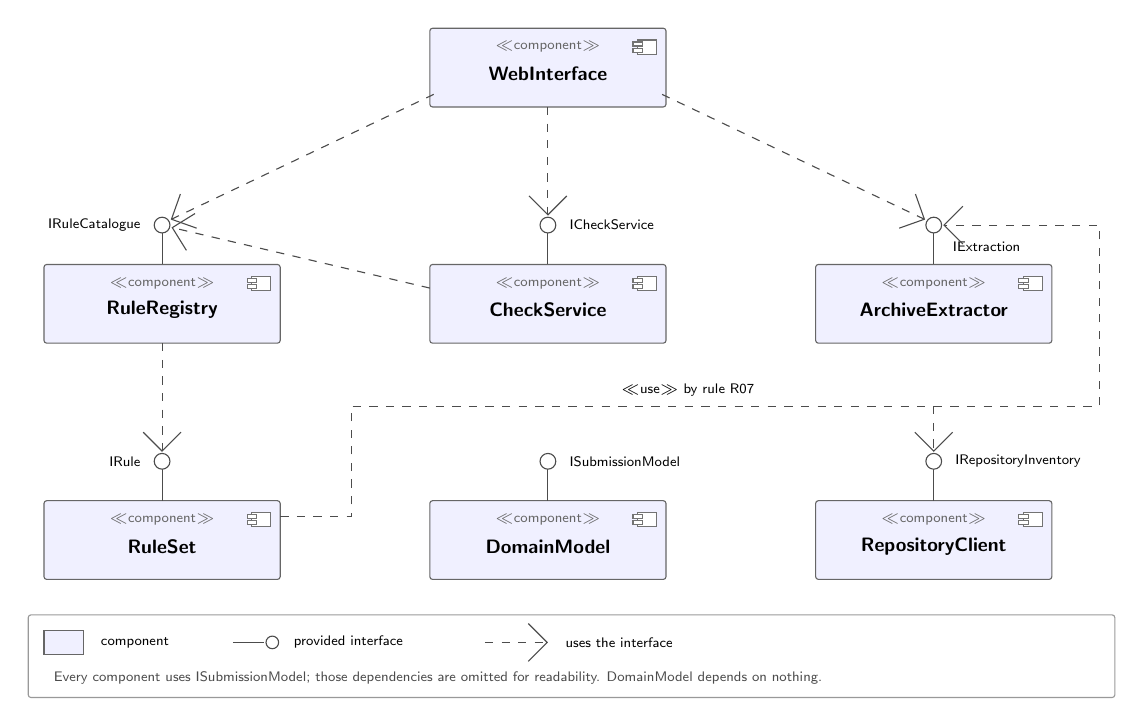
\begin{tikzpicture}[font=\scriptsize]
\foreach \cx/\cy/\name in {%
  6.5/0/WebInterface, 1.6/-3/RuleRegistry, 6.5/-3/CheckService,
  11.4/-3/ArchiveExtractor, 1.6/-6/RuleSet, 6.5/-6/DomainModel,
  11.4/-6/RepositoryClient} {
  \draw[fill=blue!6, draw=black!60, rounded corners=1pt] (\cx-1.5,\cy-0.5) rectangle (\cx+1.5,\cy+0.5);
  \node[font=\tiny, black!60] at (\cx,\cy+0.26) {$\ll$component$\gg$};
  \node[font=\scriptsize\bfseries] at (\cx,\cy-0.08) {\name};
}
\compicon{7.88}{0.26}  \compicon{2.98}{-2.74} \compicon{7.88}{-2.74}
\compicon{12.78}{-2.74} \compicon{2.98}{-5.74} \compicon{7.88}{-5.74}
\compicon{12.78}{-5.74}
\foreach \lx/\ly in {6.5/-2.5, 1.6/-2.5, 11.4/-2.5, 1.6/-5.5, 6.5/-5.5, 11.4/-5.5} {
  \draw[black!70] (\lx,\ly) -- (\lx,\ly+0.40);
  \draw[black!70, fill=white] (\lx,\ly+0.50) circle (0.10);
}
\node[font=\tiny, anchor=west] at (6.65,-2.0)   {ICheckService};
\node[font=\tiny, anchor=east] at (1.45,-2.0)   {IRuleCatalogue};
\node[font=\tiny, anchor=west] at (11.52,-2.27) {IExtraction};
\node[font=\tiny, anchor=east] at (1.45,-5.0)   {IRule};
\node[font=\tiny, anchor=west] at (6.65,-5.0)   {ISubmissionModel};
\node[font=\tiny, anchor=west] at (11.55,-5.0)  {IRepositoryInventory};
\draw[dep] (6.5,-0.5)   -- (6.5,-1.88);
\draw[dep] (5.05,-0.34) -- (1.71,-1.93);
\draw[dep] (7.95,-0.34) -- (11.29,-1.93);
\draw[dep] (5.0,-2.8)   -- (1.72,-2.03);
\draw[dep] (1.6,-3.5)   -- (1.6,-4.88);
\draw[dep] (3.1,-5.7) -- (4.0,-5.7) -- (4.0,-4.3)
  -- node[above, font=\tiny, pos=0.45] {$\ll$use$\gg$ by rule R07} (13.5,-4.3)
  -- (13.5,-2.0) -- (11.52,-2.0);
\draw[dep] (11.4,-4.3) -- (11.4,-4.88);
\begin{scope}[shift={(-0.1,-7.25)}]
  \draw[black!40, rounded corners=1pt] (0,-0.75) rectangle (13.8,0.3);
  \draw[fill=blue!6, draw=black!60] (0.2,-0.2) rectangle (0.7,0.1);
  \node[anchor=west, font=\tiny] at (0.8,-0.05) {component};
  \draw[black!70] (2.6,-0.05) -- (3.0,-0.05); \draw[black!70, fill=white] (3.1,-0.05) circle (0.08);
  \node[anchor=west, font=\tiny] at (3.25,-0.05) {provided interface};
  \draw[dep] (5.8,-0.05) -- (6.6,-0.05);
  \node[anchor=west, font=\tiny] at (6.7,-0.05) {uses the interface};
  \node[anchor=west, font=\tiny, black!70] at (0.2,-0.5)
    {Every component uses ISubmissionModel; those dependencies are omitted for readability. DomainModel depends on nothing.};
\end{scope}
\end{tikzpicture}
\caption{Component view (UML component diagram)}
\label{fig:components}
\end{figure}

Table~\ref{tab:mapping} maps every component to the module that implements it,
and the first line of each module names its component, so the architecture can
be found in the code as described \citep{Bass2021}.

\begin{table}[H]
\centering
\caption{Components and the source modules that implement them}
\label{tab:mapping}
\tablesetup
\begin{tabularx}{\textwidth}{|L{3.0cm}|L{5.8cm}|X|}
\hline
\rowcolor{gray!15}
\textbf{Component} & \textbf{Source module} & \textbf{Responsibility} \\
\hline\hline
WebInterface & \texttt{app/main.py}, \texttt{app/templates/} & Upload, report, rule catalogue, skeleton \\
\hline
CheckService & \texttt{app/checker.py} & Selects, runs and aggregates rules \\
\hline
RuleRegistry & \texttt{app/rules/base.py} & Rule interface and registration \\
\hline
RuleSet & \texttt{app/rules/naming.py}, \texttt{structure.py}, \texttt{artifacts.py}, \texttt{integrity.py}, \texttt{repository\_match.py} & Rules R01--R07 \\
\hline
DomainModel & \texttt{app/models.py} & Submission, Finding, Report; folder layout \\
\hline
ArchiveExtractor & \texttt{app/extraction.py} & Safety inspection and extraction \\
\hline
RepositoryClient & \texttt{app/repository.py} & GitHub file list and blob hashes \\
\hline
\end{tabularx}
\end{table}

\textbf{Deployment view.} Figure~\ref{fig:deployment} shows where the system runs.
The container built from the repository's Dockerfile runs as a web service on
Render; a push to the main branch triggers a new build, and the running container
reaches GitHub only through its public API. This view documents the environment
that NFR4 and NFR9 constrain \citep{Render2025}.

\begin{figure}[H]
\centering
\resizebox{\textwidth}{!}{%
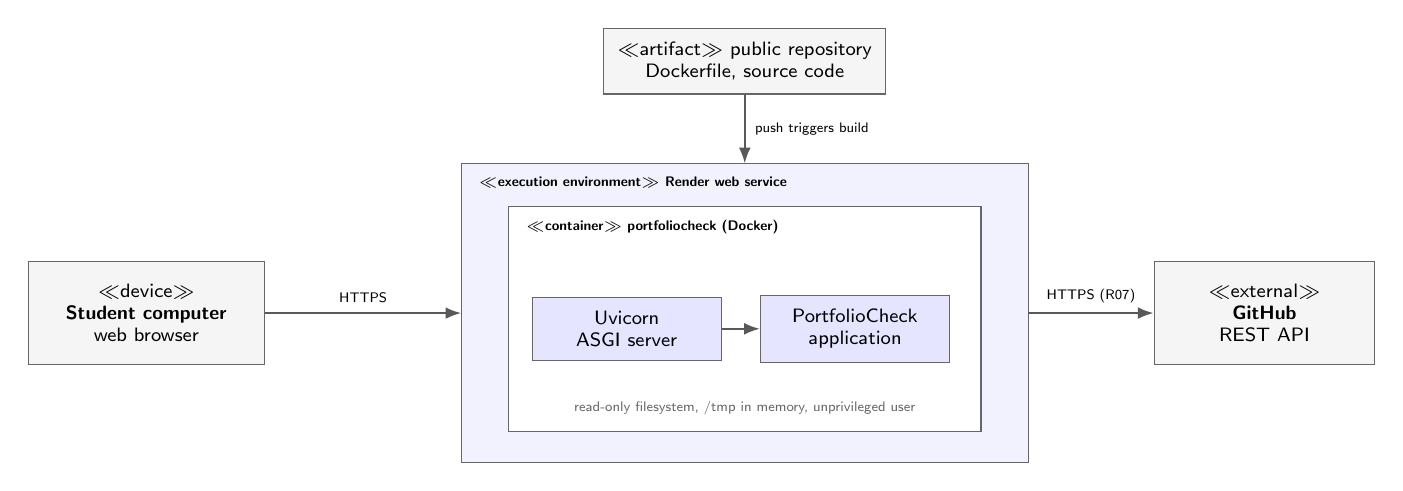
\begin{tikzpicture}[font=\scriptsize]
\node[node3d, minimum width=3.0cm, minimum height=1.3cm] (browser) at (0,0)
  {$\ll$device$\gg$\\\textbf{Student computer}\\web browser};
\draw[draw=black!60, fill=blue!5] (4.0,-1.9) rectangle (11.2,1.9);
\node[anchor=north west, font=\tiny\bfseries] at (4.1,1.85) {$\ll$execution environment$\gg$ Render web service};
\draw[draw=black!60, fill=white] (4.6,-1.5) rectangle (10.6,1.35);
\node[anchor=north west, font=\tiny\bfseries] at (4.7,1.3) {$\ll$container$\gg$ portfoliocheck (Docker)};
\node[node3d, fill=blue!10, minimum width=2.4cm] (uv) at (6.1,-0.2) {Uvicorn\\ASGI server};
\node[node3d, fill=blue!10, minimum width=2.4cm] (app) at (9.0,-0.2) {PortfolioCheck\\application};
\node[font=\tiny, black!60] at (7.6,-1.2) {read-only filesystem, /tmp in memory, unprivileged user};
\draw[flow] (uv) -- (app);
\node[node3d, minimum width=2.8cm, minimum height=1.3cm] (api) at (14.2,0) {$\ll$external$\gg$\\\textbf{GitHub}\\REST API};
\node[node3d, minimum width=2.8cm] (repo) at (7.6,3.2) {$\ll$artifact$\gg$ public repository\\Dockerfile, source code};
\draw[flow] (browser.east) -- node[above, font=\tiny] {HTTPS} (4.0,0);
\draw[flow] (11.2,0) -- node[above, font=\tiny] {HTTPS (R07)} (api.west);
\draw[flow] (repo.south) -- node[right, font=\tiny] {push triggers build} (7.6,1.9);
\end{tikzpicture}}
\caption{Deployment view (UML deployment notation)}
\label{fig:deployment}
\end{figure}

\textbf{Runtime behaviour.} The components cooperate in a fixed order when a
submission is checked. WebInterface streams the upload to a temporary folder,
stopping as soon as the size limit is reached. ArchiveExtractor inspects the
archive against the safety limits and only then extracts it, returning a
Submission. CheckService selects the rules of the chosen phase from the registry
and runs each one; each rule returns one or more findings, and rule R07
additionally asks RepositoryClient for the repository's file list. CheckService
combines all findings into a Report, WebInterface renders it, and the temporary
folder is deleted before the response leaves the server. Describing this order
explicitly matters because a structural view alone does not show it
\citep{Bass2021}.

\textbf{Architectural decisions.} Four decisions shaped the architecture more
than any other, each accepted with a known cost \citep{Ford2021}.
\textit{Rules as independent units behind a registry}: a rule can be added without
touching the engine or the interface, as the addition of R07 in the final phase
showed; the cost is the global registry recorded as TD1.
\textit{A dependency-free domain model}: every rule can be tested against an
in-memory submission in milliseconds; the cost is a small translation step where
uploaded files become a Submission \citep{Percival2020}.
\textit{No persistence}: NFR3 holds by construction and no student work is ever
stored; the cost is that no history of checks can be offered, which no
requirement asked for \citep{OWASP2021}.
\textit{The external service behind an interface that fails softly}: the core
check never depends on GitHub and R07 can be tested offline; the cost is that an
offline student gets an incomplete answer for one rule, which the report states
\citep{Newman2021}.

\textbf{Cross-cutting concepts.} Some concerns apply to every component and are
handled in one consistent way \citep{Bass2021}. \textit{Error handling} follows
two rules: an input that cannot be processed, such as a corrupt or unsafe
archive, is rejected with an explanatory page before any rule runs, while a
failure inside one rule is caught by the engine, logged and reported as a warning
for that rule alone (NFR8). \textit{Security} is concentrated at the boundary,
where every archive --- including the code archive nested inside it --- passes
the same inspection. \textit{Configuration} is limited to two environment
variables, the port and an optional GitHub token, so one container image serves
every environment. \textit{Traceability} is carried by the data itself: every
finding holds its rule identifier and the provision of the brief it comes from.

\subsection{Technology Stack}\label{sec:stack}

The application is written in Python~3.11, because archive handling and hashing
are built into its standard library \citep{PSF2025}. It uses FastAPI as web
framework, Jinja templates for the two pages, Uvicorn as server and pytest for
the tests \citep{FastAPI2025, Jinja2025, Uvicorn2025, Pytest2025}; it runs as a
Docker container on Render \citep{Docker2024, Render2025}. There is no database,
because NFR3 forbids storing submissions, and GitHub is read with the standard
library rather than a client package, because two read-only requests do not
justify a dependency. Recording the rejected options with each decision keeps it
reviewable later \citep{Ford2021}; all libraries are open source under the MIT,
BSD or Apache licence.

The web framework was the closest decision. Flask and FastAPI are both small and
would have served; FastAPI was chosen because it validates the request at the
boundary, which is exactly where untrusted uploads arrive, and because it runs
blocking work in a thread pool without extra code \citep{FastAPI2025, Flask2025}.
Django was rejected not because it is weaker but because most of what it offers
--- a database layer, migrations, an administration interface --- would have
remained unused in a system that stores nothing \citep{Django2025}. The same
reasoning ruled out a single-page front end: the interface is one form and one
report, and a separate JavaScript application would have added a second build,
a second deployment artifact and an interface contract to maintain
\citep{Richards2020}.


% =====================================================================
\section{Implementation and Evaluation}\label{sec:impl}
% =====================================================================

\subsection{Implementation}\label{sec:implementation}

The implementation grew outward from the centre of the component diagram. The
domain model came first, and one decision there shaped everything else: a finding
worse than \textit{passed} cannot be created without a corrective action, so FR8
is enforced by the type itself rather than by the care of whoever writes the next
rule \citep{Percival2020}. Archive extraction followed, deliberately before any
rule, so that no untrusted archive ever passed through an unprotected path: an
archive is rejected before anything is written to disk if it contains absolute
paths or \texttt{../} segments, more than 5,000 entries, more than 200\,MB of
content, or an entry compressed more than 200:1 --- the signatures of path
traversal and decompression bombs \citep{OWASP2021, NIST2022}.

The rules were then added one at a time, each with its test, and each designed
around the mistake students actually make \citep{Combefis2022}.
\textit{R01} checks the main folder name against the pattern
\texttt{Surname-FirstName\_MatrNo\_Course}, accepts German umlauts in names, and
only warns when the matriculation number has an unusual length, since that may be
correct. \textit{R02} checks the four required subfolders; when one is missing it
looks for a folder that differs only in case or separators, such as
\texttt{02\_requirements}, and names it, because the common mistake is a near
miss rather than an omission. \textit{R03} looks for the code archive in
\texttt{04-Implementation} and checks its name. \textit{R04} reads every
\texttt{.txt} file for a GitHub address and warns if the address of the deployed
application is missing. \textit{R05} reads the first bytes of every file ending
in \texttt{.pdf} instead of trusting the extension, because a Word file saved
under a PDF name is exactly the failure an examiner would meet. \textit{R06}
checks the 15\,MB limit and names the largest file. Rules R03, R04 and R07 apply
only to phase 3, where these artifacts are required.

The web interface came last. It discovers the rules through the registry, so the
rule catalogue on the start page stays correct as rules are added, and it runs
extraction and rule checks in a worker thread, so a slow check does not block
other users \citep{FastAPI2025}.

The last and most distinctive rule, R07, checks that the public repository and
the submitted code archive are identical. It reads the repository address from
the links file, asks the GitHub REST API for the repository's complete file tree
with the \textit{blob hash} of every file \citep{GitHubAPI2025}, and computes the
same hash for every file in the archive, so content can be compared without
downloading anything \citep{Chacon2024}. Windows line endings, the wrapper folder
added by GitHub's \textit{Download ZIP}, and macOS or \texttt{.git} metadata are
ignored so that they cause no false alarms. If GitHub cannot be reached, R07
gives a warning and all other rules still run; a private or missing repository
is a failure, because the brief requires it to be public. The code archive nested
inside the submission is untrusted in the same way as the upload itself, so it
passes the same safety inspection before any of its files is read
\citep{OWASP2021}. The result names every file that exists only in the
repository, only in the archive, or in both with different content, so the
student knows exactly what to fix.

The finished application consists of 1,136 lines of Python in twelve modules and
is accompanied by 896 lines of tests. Every module opens with a line naming the
architectural component it implements; public functions carry type annotations;
and comments explain why a decision was taken rather than repeating what the code
does. A static analysis with pyflakes reports no defects other than the
deliberate registry imports recorded as TD1. Code that is small, typed and
self-explaining matters most in a project that will be read by someone other
than its author, such as an examiner \citep{Winters2020}.

\subsection{Testing}\label{sec:testing}

Testing combined manual test cases with an automated suite. Table~\ref{tab:manual}
specifies each manual test case by its exact input and expected behaviour, as the
Phase~2 feedback requested; specifying tests this way makes them repeatable by
someone other than their author \citep{Winters2020}. Inputs M01--M09 are
realistic sample submissions for a fictional project, generated by a script, each
differing from the compliant one in exactly one respect so that each case tests
exactly one rule; they use the example name from the brief so that no real
person's data appears in the repository \citep{NIST2022}. Cases M10--M13 use the
real project repository. Every case is run by choosing the file and phase on the
start page and pressing \textit{Check submission}; Appendix~A shows the actual
output of the application for each of the cases M01--M09.

\begin{table}[H]
\centering
\caption{Manual test cases with input, expected behaviour and result}
\label{tab:manual}
\tablesetup
\begin{tabularx}{\textwidth}{|c|L{4.6cm}|c|X|c|}
\hline
\rowcolor{gray!15}
\textbf{ID} & \textbf{Input} & \textbf{Ph.} & \textbf{Expected behaviour} & \textbf{Result} \\
\hline\hline
M01 & \texttt{M01}: compliant submission & 1 & \textit{Ready to submit}; R01, R02, R05, R06 pass & Pass \\
\hline
M02 & \texttt{M02}: main folder \nolinkurl{Mustermann_Max_12345678_PSE} & 1 & R01 fail: \textit{does not follow the required pattern} & Pass \\
\hline
M03 & \texttt{M03}: folder \nolinkurl{02_requirements} & 1 & R02 fail: \textit{A folder named '02\_requirements' exists} & Pass \\
\hline
M04 & \texttt{M04}: matriculation number \texttt{123456} & 1 & \textit{Almost there}; R01 warn: \textit{is not 8 digits long} & Pass \\
\hline
M05 & \texttt{M05}: Word file saved as \nolinkurl{architecture.pdf} & 2 & R05 fail: \textit{has a .pdf extension but is not a PDF file} & Pass \\
\hline
M06 & \texttt{M06}: code archive named \texttt{code.zip} & 3 & R03 fail: \textit{No correctly named code archive} & Pass \\
\hline
M07 & \texttt{M07}: links file without application URL & 3 & R04 warn: \textit{contains no second URL for the deployed application} & Pass \\
\hline
M08 & \texttt{M08}: entry \nolinkurl{../outside-the-upload-folder.txt} & any & Error page: \textit{Unsafe path in archive}; nothing extracted & Pass \\
\hline
M09 & \texttt{M09}: text file renamed to \texttt{.zip} & any & Error page: \textit{not a valid ZIP archive} & Pass \\
\hline
M10 & Phase~3 submission; code archive made from the repository with \texttt{git archive} & 3 & R07 pass: \textit{All N files \ldots\ are identical} & Pass \\
\hline
M11 & As M10, one line of \nolinkurl{app/main.py} changed in the code archive only & 3 & R07 fail naming \nolinkurl{app/main.py} & Pass \\
\hline
M12 & As M10, links file naming a repository that is not publicly visible & 3 & R07 fail: \textit{does not exist or is not public} & Pass \\
\hline
M13 & As M10, GitHub unreachable (connection refused) & 3 & R07 warn: \textit{GitHub could not be reached} & Pass \\
\hline
\end{tabularx}
\end{table}

Cases M10 to M13 test R07 against the real repository and were run after
deployment, M10 to M12 on the deployed application itself. For M10, the code
archive was created from the current state of the repository, and the check
confirmed that all 66 files are identical. M11 changes one line of a source file
in the archive only, and the check named exactly that file. M12 names a repository
address that GitHub does not serve publicly; GitHub answers a private and a
non-existent repository with the same response, so this case covers both. M13 was
run locally with every connection to GitHub refused; R07 degraded to a warning
while the other six rules still produced their findings. Together these four
cases exercise every outcome of R07 on real data rather than on the simulation
used in the automated tests \citep{Winters2020}.

The test data was designed with three properties. Each sample differs from the
compliant one in exactly one respect, so a failure can only have one cause. The
samples are generated by a script rather than assembled by hand, and the script
fixes all timestamps, so every run produces byte-identical archives that can be
reviewed and recreated. And the documents inside the samples are valid PDF files
with meaningful text about a fictional study-room booking project, as the brief
requires sensible test data rather than placeholder content. Test data that is
realistic, minimal in its variation and itself under test is what makes a test
result convincing \citep{Khorikov2020}.

The automated suite contains 73 tests in five modules. The 23 \textit{rule
tests} exercise every rule against a compliant submission and against one that
violates exactly that rule; they also include a resilience test, in which a
deliberately broken rule is added and the remaining rules must still produce
their findings (NFR8), and a timing test for NFR5. The 5 \textit{extraction
tests} feed crafted archives to every safety limit: a path with \texttt{../}, an
absolute path, 5,001 entries and a 50\,MB file compressed to a few kilobytes. The
23 \textit{repository tests} check R07 against a simulated GitHub that can be told
to succeed, to report a missing repository, to hit the rate limit or to be
unreachable, so no test depends on the network; three of them confirm that the
computed hashes equal those of \texttt{git hash-object}. The 10 \textit{interface
tests} exercise the whole path from upload to report, including the error pages,
and the 12 \textit{sample tests} confirm that every input of
Table~\ref{tab:manual} produces the documented result \citep{Khorikov2020}. The last group ties the manual and the automated tests
together: the expected results in Table~\ref{tab:manual} are themselves executed
on every run, so the specification cannot drift away from the behaviour of the
application. Figure~\ref{fig:pytest} in Appendix~A shows a complete run in which all 73 tests
pass; the suite was also run from a clean extraction of the submission archive
to confirm that the published code is self-contained \citep{Pytest2025}.

\subsection{Results}\label{sec:results}

Figure~\ref{fig:start} in Appendix~A shows the start page of the running
application. It
offers the upload form and the phase selection, and it lists every rule with the
provision of the brief behind it, so a student knows exactly what will be checked
before uploading anything (FR13). The link below the form downloads an empty,
correctly named folder structure for students starting from nothing (FR10)
\citep{Sommerville2020}.

Figure~\ref{fig:report} shows the report for sample M05 checked as phase 3. The
headline says the submission is not ready and counts three problems to fix, one
to review and three passed rules. The Word file saved as
\texttt{architecture.pdf} is caught by R05; because the sample is a phase-2
folder, the code archive and links file that phase 3 requires are missing, so
R03 and R04 fail, and R07 explains that the repository comparison could not run
until those are fixed. Failures come first, each with its correction and the
chapter of the brief it derives from (FR8, FR11), which is the behaviour the
project set out to deliver \citep{Messer2024}.

\begin{figure}[!htbp]
\centering
\screenshot{screenshots/report_M05.jpg}{0.5\textwidth}{Report for M05}
\caption{Report for sample M05 checked as phase 3}
\label{fig:report}
\end{figure}

Measured against the four objectives of Section~\ref{sec:profile}, the result is
as follows. Every formal provision of the brief that can be checked mechanically
is covered by one of the seven rules; the only provisions left out are the
typographic rules for the abstract, which would require parsing page layout.
Every failure carries its correction, which the domain model enforces. Without
the GitHub comparison a typical submission is checked in well under a second, as
the timing test confirms; in phase 3 the two GitHub requests are bounded by a
timeout of 2.5 seconds, after which R07 reports a warning instead of waiting. And the application is reachable in a browser
without installation or login \citep{Sommerville2020}.

All thirteen functional requirements are implemented, including the optional
FR12, and each is verified by an automated test and, where visible in the
interface, by a manual test case (Table~\ref{tab:requirements}). Of the
non-functional requirements, NFR1, NFR2, NFR5 and NFR8 are verified by automated
tests, NFR3 and NFR4 by review of the code and the container configuration, NFR6
by the manual test cases, NFR7 by the addition of R07, which needed a new rule
module and a new client module but no change to the engine or the interface, and
NFR9 by the cloud deployment \citep{ISO25010}.

The tool also has limits, stated here rather than left for users to discover.
Its rules encode the brief of one course; the PDF rule confirms that a file is a
PDF but not that it opens cleanly; the repository check depends on GitHub; and
the tool checks form, not content, so a submission that passes every rule can
still fail its assessment. The interface says so on every page, because a
compliance tool mistaken for a quality tool would do more harm than good
\citep{Messer2024}.

\subsection{Deployment and Installation}\label{sec:deployment}

The application runs as a Render web service built from the repository's
Dockerfile and blueprint file; the port is taken from the environment, so the
same image runs locally and in the cloud \citep{Render2025, Docker2024}. No login
is required: a student opens the address, chooses the zip folder and the phase,
and presses \textit{Check submission}. The free tier pauses the service after a
period of inactivity, so the first request afterwards can take up to a minute;
this is noted in the links file for the examiner.

For local use the README in the repository gives two procedures. With Docker, a
single command, \texttt{docker compose up --build}, builds and starts the
container, which then serves the application at \texttt{http://localhost:8000}.
Without Docker, a Python 3.11 virtual environment is created, the dependencies
are installed from \texttt{requirements.txt}, and the server is started with
\texttt{uvicorn app.main:app}; the tests run with \texttt{python -m pytest}. An
optional \texttt{GITHUB\_TOKEN} environment variable raises the GitHub rate limit
used by R07. Keeping installation to one command is what makes the application
usable by an examiner without assistance \citep{Kim2021}.

\begin{itemize}[itemsep=0pt]
\item \textbf{Application:} \url{https://portfoliocheck-bwwq.onrender.com}
\item \textbf{Repository:} \url{https://github.com/shivakondaru94-gif/portfoliocheck-DLMCSPSE01}
\end{itemize}

Figure~\ref{fig:render} in Appendix~A shows the service running live on
Render.

% =====================================================================
\section{Reflection}\label{sec:reflection}
% =====================================================================

\subsection{Technical Debt}\label{sec:debt}

Technical debt means shortcuts in the implementation that saved time at the cost
of internal quality and that, like financial debt, should be repaid before the
interest grows \citep{Avgeriou2023}. It is not a list of missing features; all
functional requirements are implemented. Table~\ref{tab:debt} lists the debt that
remains, ordered by its effect on maintenance \citep{Lenarduzzi2021}.

\begin{table}[H]
\centering
\caption{Open technical debt}
\label{tab:debt}
\tablesetup
\begin{tabularx}{\textwidth}{|c|L{4.4cm}|X|L{3.4cm}|}
\hline
\rowcolor{gray!15}
\textbf{ID} & \textbf{Shortcut} & \textbf{Consequence} & \textbf{Repayment} \\
\hline\hline
TD1 & Rule registry is a global list filled by import side effects & A rule module not imported is silently inactive; tests must patch shared instances & Explicit registry object created at start-up \\
\hline
TD2 & Limits hard-coded as constants in four modules & Changing a limit needs a code change and redeployment & One settings object read from the environment \\
\hline
TD3 & GitHub responses not cached & Without a token, about 30 phase-3 checks per hour before R07 degrades & Short-lived cache per repository \\
\hline
TD4 & PDF check reads only the file header & A corrupt PDF with a valid header passes R05 & Parse each PDF with a PDF library \\
\hline
TD5 & R07 repeats the link and archive lookup of R03 and R04 & The three rules could disagree after one is changed & Shared lookup functions \\
\hline
TD6 & Interface tests check HTML text & A purely visual change can break tests & JSON report for tests \\
\hline
TD7 & Messages written as English strings inside rule classes & Rewording or translating means editing rule logic & Message catalogue \\
\hline
\end{tabularx}
\end{table}

The order of the table reflects the cost of leaving each item in place. TD1 and
TD2 come first because they affect every future change: any new rule depends on
the registry, and any new deployment depends on the limits. TD3 matters as soon
as the application is shared by many students before a deadline. TD4 to TD7 are
local and can be repaid independently when the affected part is next changed. This
order follows the common practice of prioritising debt by how much further work
it makes more expensive \citep{Lenarduzzi2021}.

Three items were repaid during the project: a duplicated regular expression was
moved into a shared module, blocking work on the request thread was moved to a
worker thread before R07 added network calls, and the untested error path of the
rule engine received a test \citep{Winters2020}.

\subsection{Lessons Learned}\label{sec:lessons}

\textit{Tools.} Treating the standard library as the first choice kept the code
that handles untrusted input free of third-party dependencies
\citep{PSF2025}, and git's own content hashes proved the right way to compare
repository and archive; comparing file sizes would have missed edits that keep a
file's length \citep{Chacon2024}. The Kanban board, by contrast, was first drawn
instead of kept in a tool, and the Phase~2 feedback showed why that was wrong: a
drawing shows intentions, while a board linked to commits shows what happened
\citep{GitHubProjects2025}.

\textit{Method.} Working on one work package at a time mattered more than
expected, because it stopped the rule set from growing faster than its tests
\citep{Ambler2022}. Writing each test together with its rule meant that the late
addition of R07 could not break R01--R06 unnoticed, and building the extraction
defences before any rule meant they never had to be added afterwards
\citep{Khorikov2020}. The tutorial feedback proved as valuable as the
development loop itself: it corrected the architecture notation, the meaning of
technical debt and the way test cases are written \citep{Schwaber2020}.

\textit{Time.} The single external dependency, R07, took the largest share of the
final phase, as the risk register had predicted. Isolating it behind an interface
early meant the rest of the system never waited for it and that it could be
tested fully without the network, and scheduling it first in the phase left time
for deployment \citep{Sommerville2020}.

\textit{What would be done differently.} Three things would change in a second
attempt. The board would live in a tool from the first day, because its evidence
only accumulates while it is in use. The rule registry would be an explicit
object from the start; the global list was quicker to write but is now the first
item of technical debt, and replacing it later costs more than building it
properly would have. And the manual test cases would be written in their final,
concrete form during the conception phase rather than as general test levels,
since concrete inputs and expected outputs expose unclear requirements earlier
\citep{Avgeriou2023, Winters2020}.

\subsection{Conclusion}\label{sec:conclusion}

PortfolioCheck addresses a narrow and practically unaddressed problem: formal
submission requirements are mechanical and carry marks, yet they are checked by
hand at the least favourable moment. The finished application checks seven rules
derived from the brief, explains every failure with its correction and source,
and verifies that repository and code archive are identical --- a provision that
cannot practically be checked by hand. All functional requirements are
implemented, every quality requirement has recorded evidence, and the
architecture documented here is the one found in the code \citep{Bass2021}. The
most useful next steps follow from the technical debt: an explicit registry and
external configuration would let the rules be adapted to other courses, and a
cache for repository data would let one deployment serve a whole cohort in the
days before a deadline \citep{Ford2021}.

\newpage

% =====================================================================
% REFERENCES
% =====================================================================
\clearpage
\addcontentsline{toc}{section}{References}

\begin{thebibliography}{99}
\setlength{\itemsep}{4pt}
\small

\bibitem[Ambler and Lines(2022)]{Ambler2022}
Ambler, S. W. and Lines, M. (2022) \textit{Choose Your WoW! A Disciplined Agile
Approach to Optimizing Your Way of Working}. 2nd edn. Newtown Square, PA:
Project Management Institute.

\bibitem[Avgeriou et~al.(2023)]{Avgeriou2023}
Avgeriou, P., Ozkaya, I., Chatzigeorgiou, A., Ciolkowski, M., Ernst, N. A.,
Koontz, R. J., Poort, E. and Shull, F. (2023) `Technical debt management: the
road ahead for successful software delivery', in \textit{2023 IEEE/ACM
International Conference on Software Engineering: Future of Software Engineering
(ICSE-FoSE)}, pp. 15--30.

\bibitem[Bass et~al.(2021)]{Bass2021}
Bass, L., Clements, P. and Kazman, R. (2021) \textit{Software Architecture in
Practice}. 4th edn. Boston, MA: Addison-Wesley.

\bibitem[Brown(2024)]{Brown2024}
Brown, S. (2024) \textit{The C4 Model for Visualising Software Architecture}.
Available at: \url{https://c4model.com/} (Accessed: 1 October 2026).

\bibitem[Chacon and Straub(2024)]{Chacon2024}
Chacon, S. and Straub, B. (2024) \textit{Pro Git}. 2nd edn (continuously
updated). Available at: \url{https://git-scm.com/book/} (Accessed: 1 October 2026).

\bibitem[Comb\'{e}fis(2022)]{Combefis2022}
Comb\'{e}fis, S. (2022) `Automated code assessment for education: review,
classification and perspectives on techniques and tools', \textit{Software},
1(1), pp. 3--30.

\bibitem[Django Software Foundation(2025)]{Django2025}
Django Software Foundation (2025) \textit{Django Documentation}. Available at:
\url{https://docs.djangoproject.com/} (Accessed: 1 October 2026).

\bibitem[Docker(2024)]{Docker2024}
Docker Inc. (2024) \textit{Compose Specification}. Available at:
\url{https://docs.docker.com/compose/} (Accessed: 1 October 2026).

\bibitem[Encode(2025)]{Uvicorn2025}
Encode (2025) \textit{Uvicorn: An ASGI Web Server for Python}. Available at:
\url{https://www.uvicorn.org/} (Accessed: 1 October 2026).

\bibitem[Ford et~al.(2021)]{Ford2021}
Ford, N., Richards, M., Sadalage, P. and Dehghani, Z. (2021) \textit{Software
Architecture: The Hard Parts --- Modern Trade-Off Analyses for Distributed
Architectures}. Sebastopol, CA: O'Reilly Media.

\bibitem[GitHub(2025a)]{GitHubAPI2025}
GitHub Inc. (2025) \textit{REST API Endpoints for Git Trees}. GitHub Docs.
Available at: \url{https://docs.github.com/en/rest/git/trees} (Accessed: 1 October 2026).

\bibitem[GitHub(2025b)]{GitHubProjects2025}
GitHub Inc. (2025) \textit{About Projects}. GitHub Docs. Available at:
\url{https://docs.github.com/en/issues/planning-and-tracking-with-projects}
(Accessed: 1 October 2026).

\bibitem[Hermans(2021)]{Hermans2021}
Hermans, F. (2021) \textit{The Programmer's Brain: What Every Programmer Needs
to Know about Cognition}. Shelter Island, NY: Manning.

\bibitem[ISO/IEC(2023)]{ISO25010}
International Organization for Standardization (2023) \textit{ISO/IEC
25010:2023 Systems and Software Engineering --- Systems and Software Quality
Requirements and Evaluation (SQuaRE) --- Product Quality Model}. Geneva: ISO.

\bibitem[Khorikov(2020)]{Khorikov2020}
Khorikov, V. (2020) \textit{Unit Testing Principles, Practices, and Patterns}.
Shelter Island, NY: Manning.

\bibitem[Kim et~al.(2021)]{Kim2021}
Kim, G., Humble, J., Debois, P., Willis, J. and Forsgren, N. (2021) \textit{The
DevOps Handbook}. 2nd edn. Portland, OR: IT Revolution Press.

\bibitem[Lenarduzzi et~al.(2021)]{Lenarduzzi2021}
Lenarduzzi, V., Besker, T., Taibi, D., Martini, A. and Arcelli Fontana, F.
(2021) `A systematic literature review on technical debt prioritization:
strategies, processes, factors, and tools', \textit{Journal of Systems and
Software}, 171, 110827.

\bibitem[Messer et~al.(2024)]{Messer2024}
Messer, M., Brown, N. C. C., K\"{o}lling, M. and Shi, M. (2024) `Automated
grading and feedback tools for programming education: a systematic review',
\textit{ACM Transactions on Computing Education}, 24(1), pp. 1--43.

\bibitem[Newman(2021)]{Newman2021}
Newman, S. (2021) \textit{Building Microservices: Designing Fine-Grained
Systems}. 2nd edn. Sebastopol, CA: O'Reilly Media.

\bibitem[NIST(2022)]{NIST2022}
National Institute of Standards and Technology (2022) \textit{SP 800-218:
Secure Software Development Framework (SSDF) Version 1.1}. Gaithersburg, MD: NIST.

\bibitem[OWASP(2021)]{OWASP2021}
Open Worldwide Application Security Project (2021) \textit{OWASP Top 10:2021}.
Available at: \url{https://owasp.org/Top10/} (Accessed: 1 October 2026).

\bibitem[Paiva et~al.(2022)]{Paiva2022}
Paiva, J. C., Leal, J. P. and Figueira, \'{A}. (2022) `Automated assessment in
computer science education: a state-of-the-art review', \textit{ACM
Transactions on Computing Education}, 22(3), pp. 1--40.

\bibitem[Pallets(2025a)]{Flask2025}
Pallets Projects (2025) \textit{Flask Documentation}. Available at:
\url{https://flask.palletsprojects.com/} (Accessed: 1 October 2026).

\bibitem[Pallets(2025b)]{Jinja2025}
Pallets Projects (2025) \textit{Jinja Documentation}. Available at:
\url{https://jinja.palletsprojects.com/} (Accessed: 1 October 2026).

\bibitem[Percival and Gregory(2020)]{Percival2020}
Percival, H. and Gregory, B. (2020) \textit{Architecture Patterns with Python}.
Sebastopol, CA: O'Reilly Media.

\bibitem[pytest-dev(2025)]{Pytest2025}
pytest-dev Team (2025) \textit{pytest Documentation}. Available at:
\url{https://docs.pytest.org/} (Accessed: 1 October 2026).

\bibitem[Python Software Foundation(2025)]{PSF2025}
Python Software Foundation (2025) \textit{zipfile --- Work with ZIP Archives}.
Python 3.11 Standard Library Documentation. Available at:
\url{https://docs.python.org/3/library/zipfile.html} (Accessed: 1 October 2026).

\bibitem[Ram\'{i}rez(2025)]{FastAPI2025}
Ram\'{i}rez, S. (2025) \textit{FastAPI Documentation}. Available at:
\url{https://fastapi.tiangolo.com/} (Accessed: 1 October 2026).

\bibitem[Render(2025)]{Render2025}
Render Services Inc. (2025) \textit{Render Documentation: Docker and Blueprints}.
Available at: \url{https://render.com/docs} (Accessed: 1 October 2026).

\bibitem[Richards and Ford(2020)]{Richards2020}
Richards, M. and Ford, N. (2020) \textit{Fundamentals of Software Architecture:
An Engineering Approach}. Sebastopol, CA: O'Reilly Media.

\bibitem[Schwaber and Sutherland(2020)]{Schwaber2020}
Schwaber, K. and Sutherland, J. (2020) \textit{The Scrum Guide: The Definitive
Guide to Scrum}. Available at: \url{https://scrumguides.org/} (Accessed: 1 October 2026).

\bibitem[Sommerville(2020)]{Sommerville2020}
Sommerville, I. (2020) \textit{Engineering Software Products: An Introduction
to Modern Software Engineering}. Harlow: Pearson Education.

\bibitem[Winters et~al.(2020)]{Winters2020}
Winters, T., Manshreck, T. and Wright, H. (2020) \textit{Software Engineering
at Google: Lessons Learned from Programming over Time}. Sebastopol, CA: O'Reilly Media.

\end{thebibliography}

% =====================================================================
% APPENDIX A -- WORKING RESULTS
% =====================================================================
\newpage
\appendix
\section*{Appendix A: Working Results}
\addcontentsline{toc}{section}{Appendix A: Working Results}
\label{app:results}
\setcounter{figure}{0}
\renewcommand{\thefigure}{A.\arabic{figure}}
\renewcommand{\theHfigure}{A.\arabic{figure}}

This appendix shows the application at work for the manual test cases of
Table~\ref{tab:manual}, so that each result recorded there as \textit{Pass} can be
seen. Each screenshot was taken on a laptop of the complete browser window while
the application was running locally: the sample submission named in the caption
was uploaded through the start page with the phase given in the table, and the
address bar shows the page the application returned. For long reports the window
shows the top of the page, where the failures are listed first. Case M05 is shown
in Figure~\ref{fig:report}. The phase-3 samples M06 and M07 link to the example
repository address from the assignment brief, which does not exist, so rule R07
reports a failure for them, as documented in the repository's sample
description. The appendix also shows the start page, the run of the automated test suite
and the deployed service.

\begin{figure}[H]
\centering
\screenshot{screenshots/start_page.jpg}{0.62\textwidth}{Start page}
\caption{Start page with upload form and rule catalogue}
\label{fig:start}
\end{figure}

\begin{figure}[H]
\centering
\fbox{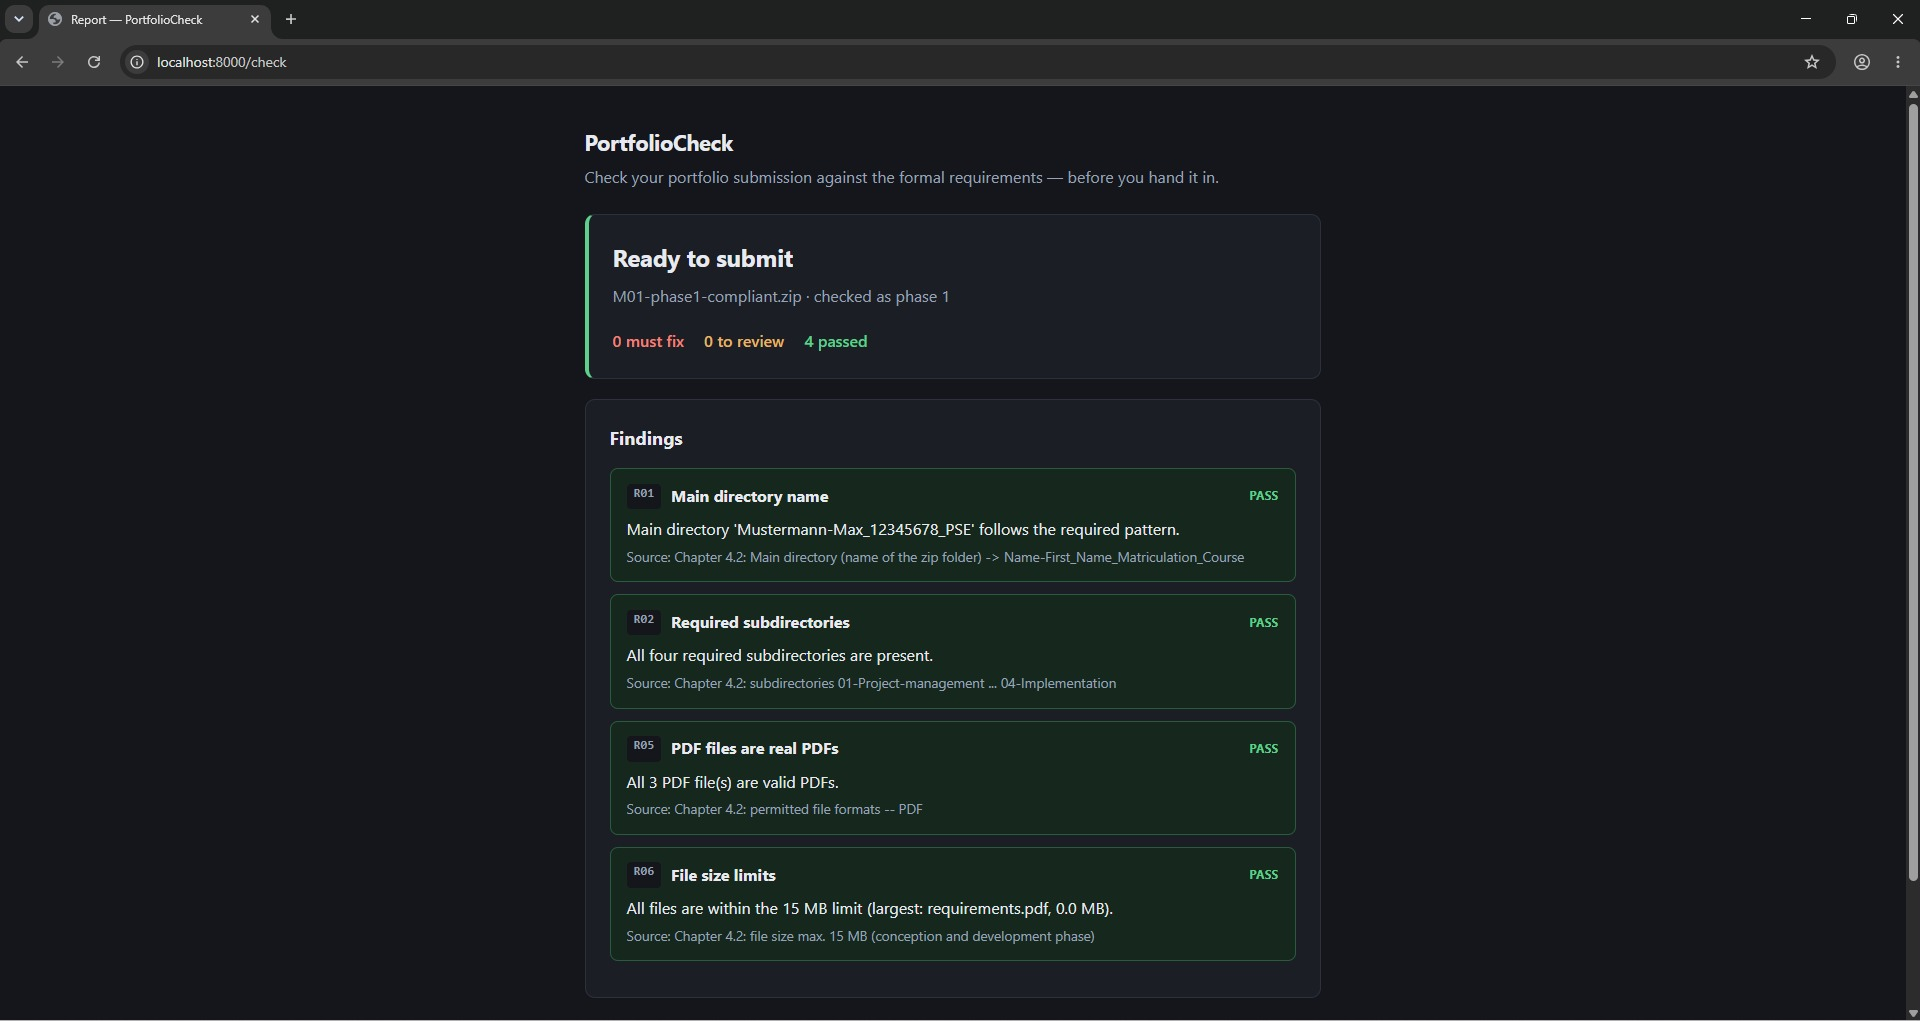
\includegraphics[width=0.97\textwidth]{screenshots/appendix/M01_compliant.jpg}}
\caption{M01, phase 1: compliant submission --- \textit{Ready to submit}}
\end{figure}

\begin{figure}[H]
\centering
\fbox{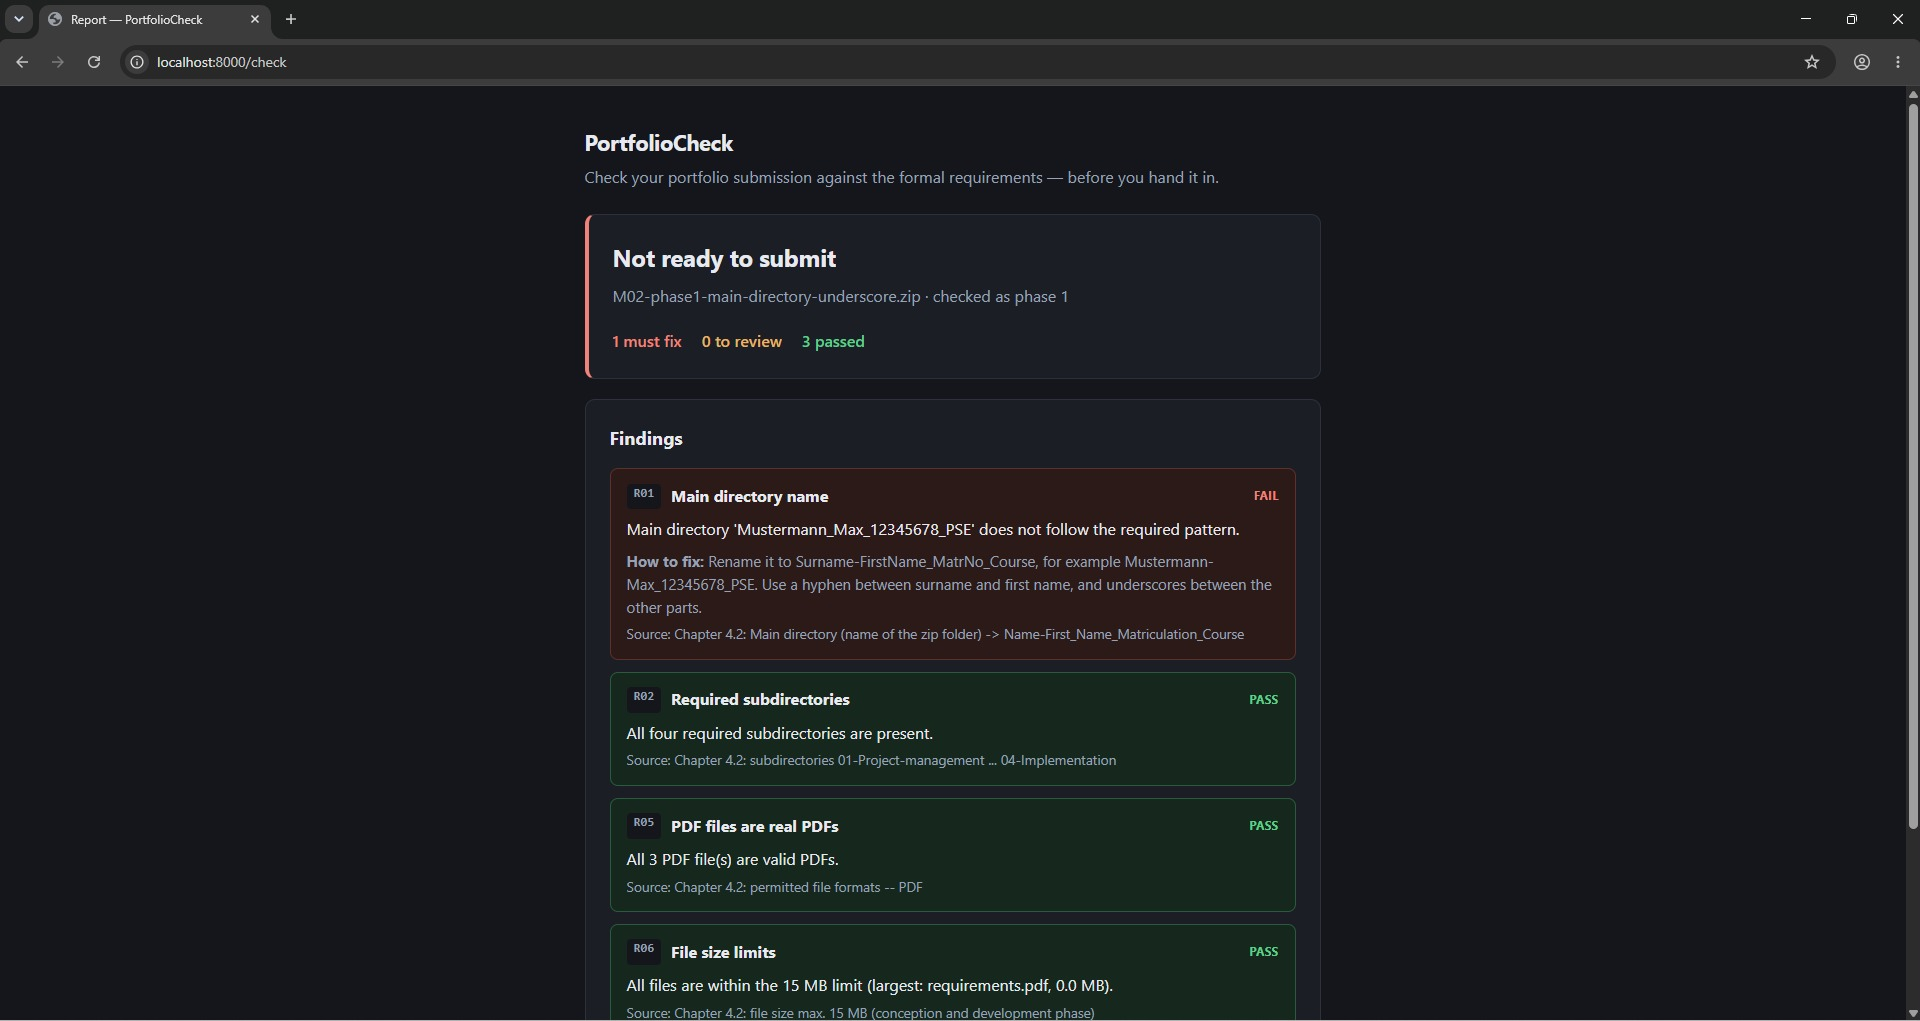
\includegraphics[width=0.97\textwidth]{screenshots/appendix/M02_main_directory_underscore.jpg}}
\caption{M02, phase 1: underscore in the main directory name --- R01 fails}
\end{figure}

\begin{figure}[H]
\centering
\fbox{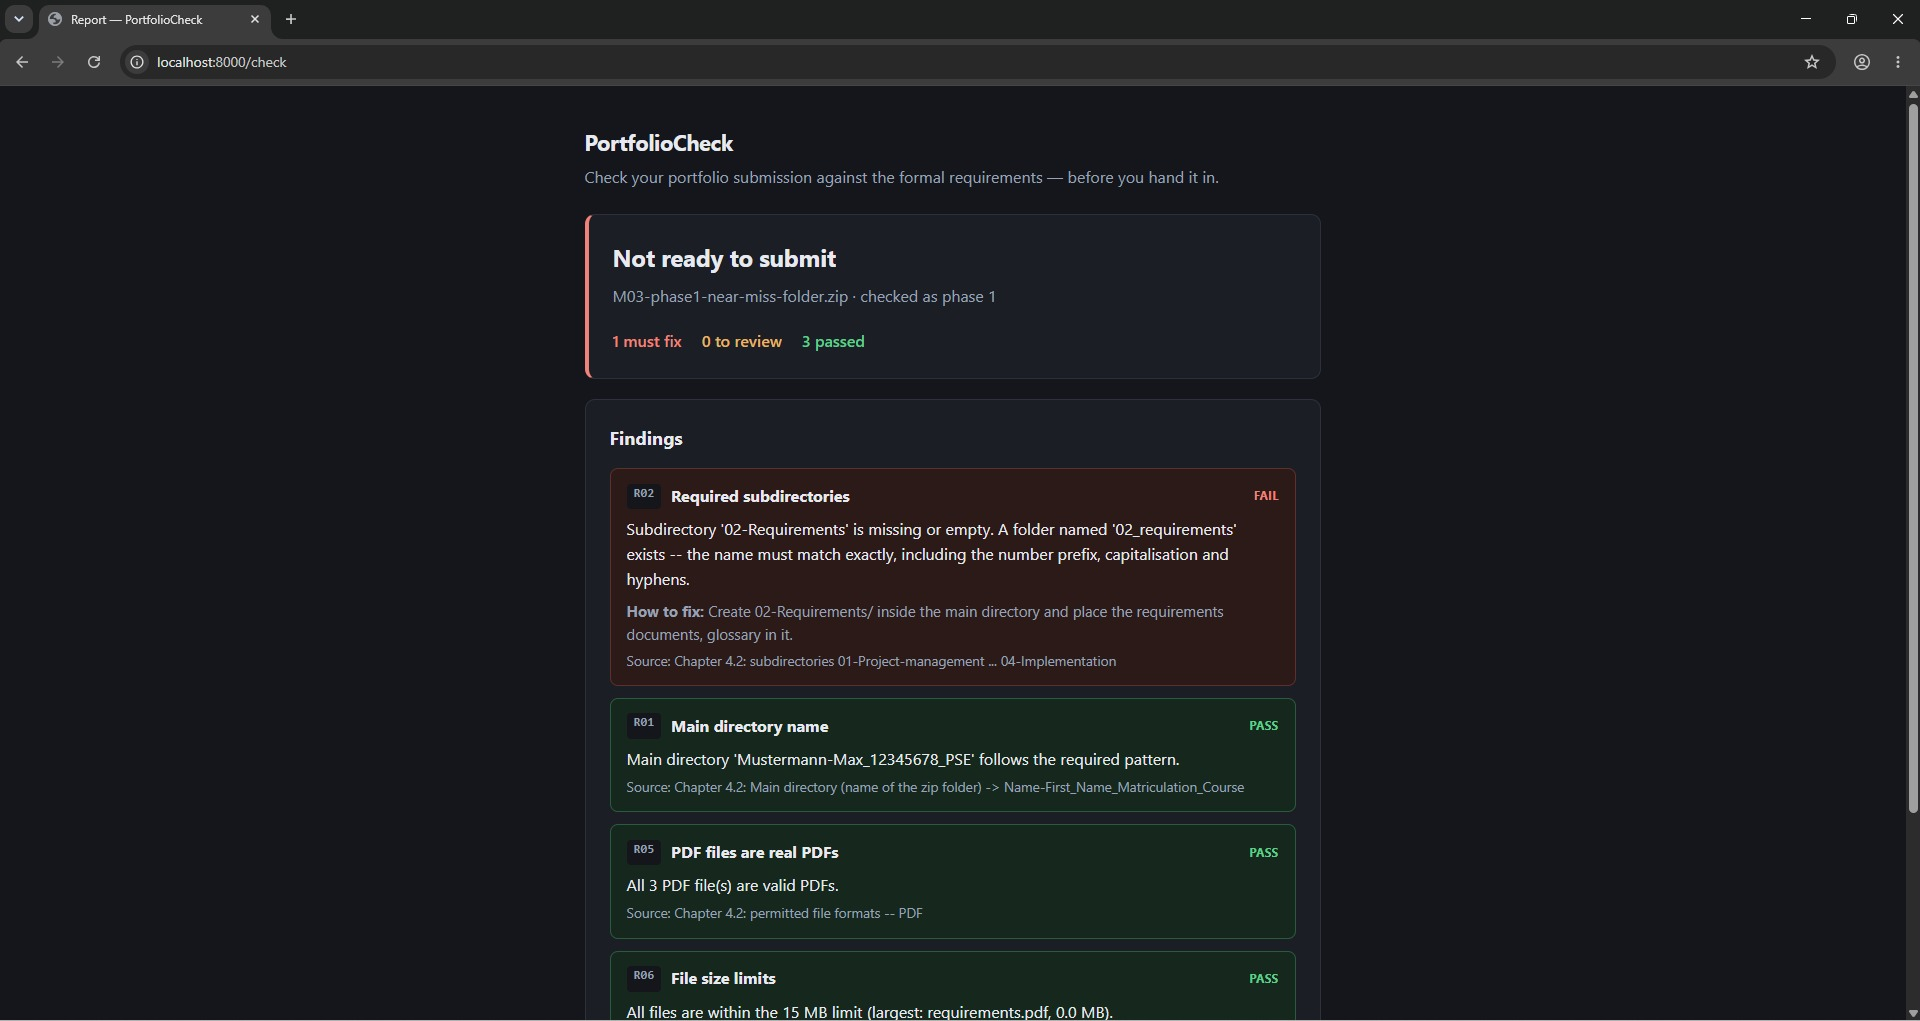
\includegraphics[width=0.97\textwidth]{screenshots/appendix/M03_near_miss_folder.jpg}}
\caption{M03, phase 1: folder \texttt{02\_requirements} --- R02 fails and names it}
\end{figure}

\begin{figure}[H]
\centering
\fbox{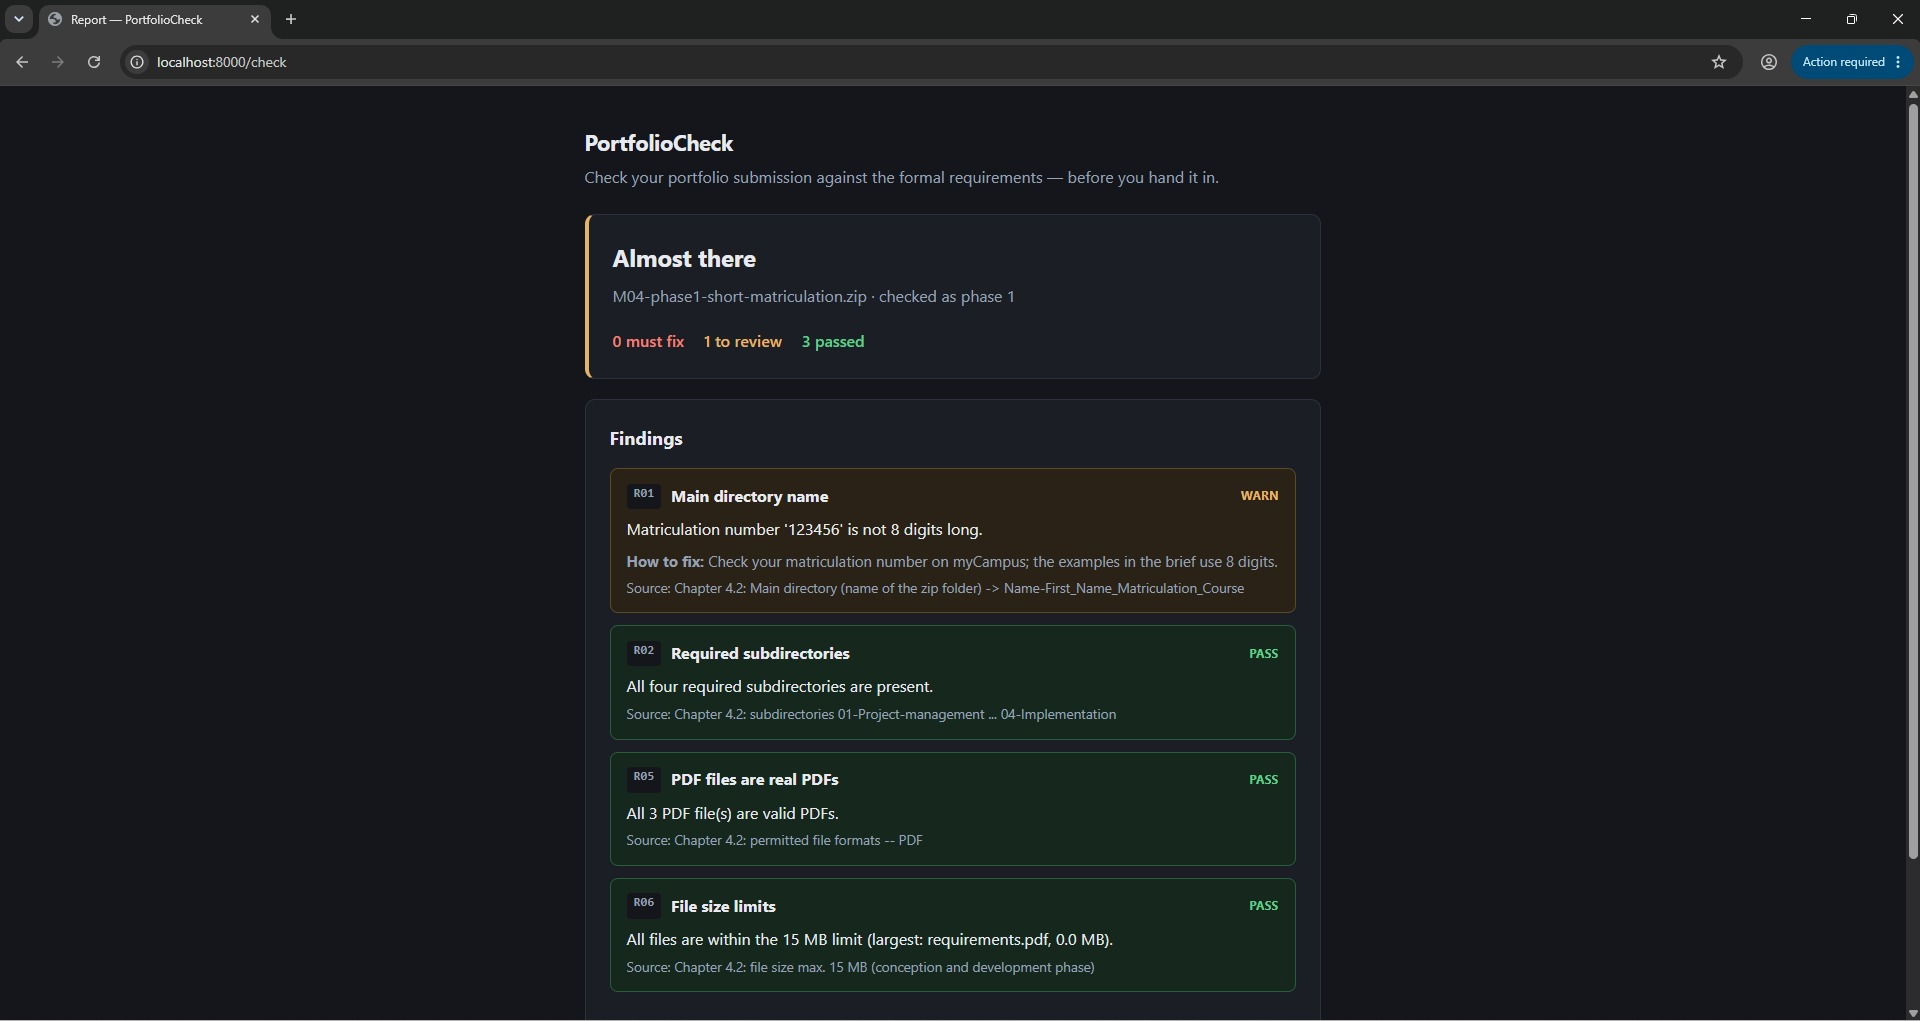
\includegraphics[width=0.97\textwidth]{screenshots/appendix/M04_short_matriculation.jpg}}
\caption{M04, phase 1: six-digit matriculation number --- R01 warns, \textit{Almost there}}
\end{figure}

\begin{figure}[H]
\centering
\fbox{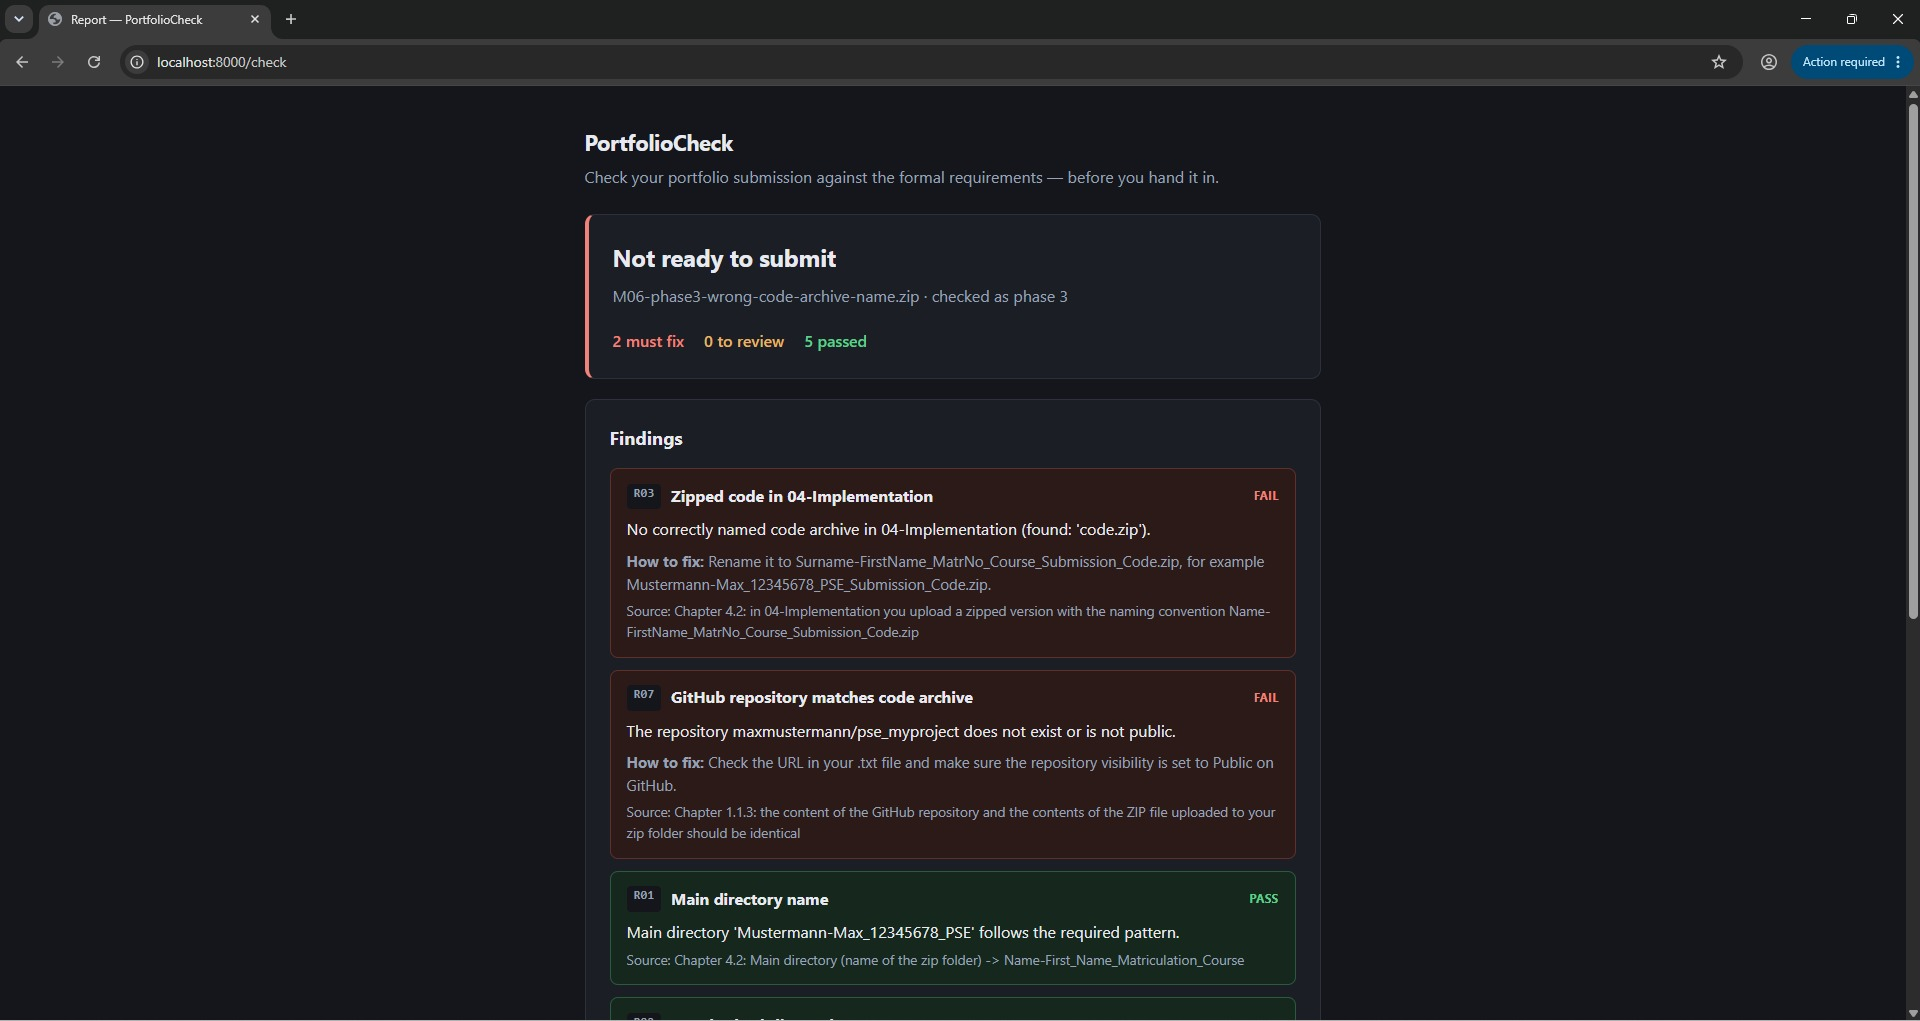
\includegraphics[width=0.97\textwidth]{screenshots/appendix/M06_wrong_code_archive_name.jpg}}
\caption{M06, phase 3: code archive named \texttt{code.zip} --- R03 fails}
\end{figure}

\begin{figure}[H]
\centering
\fbox{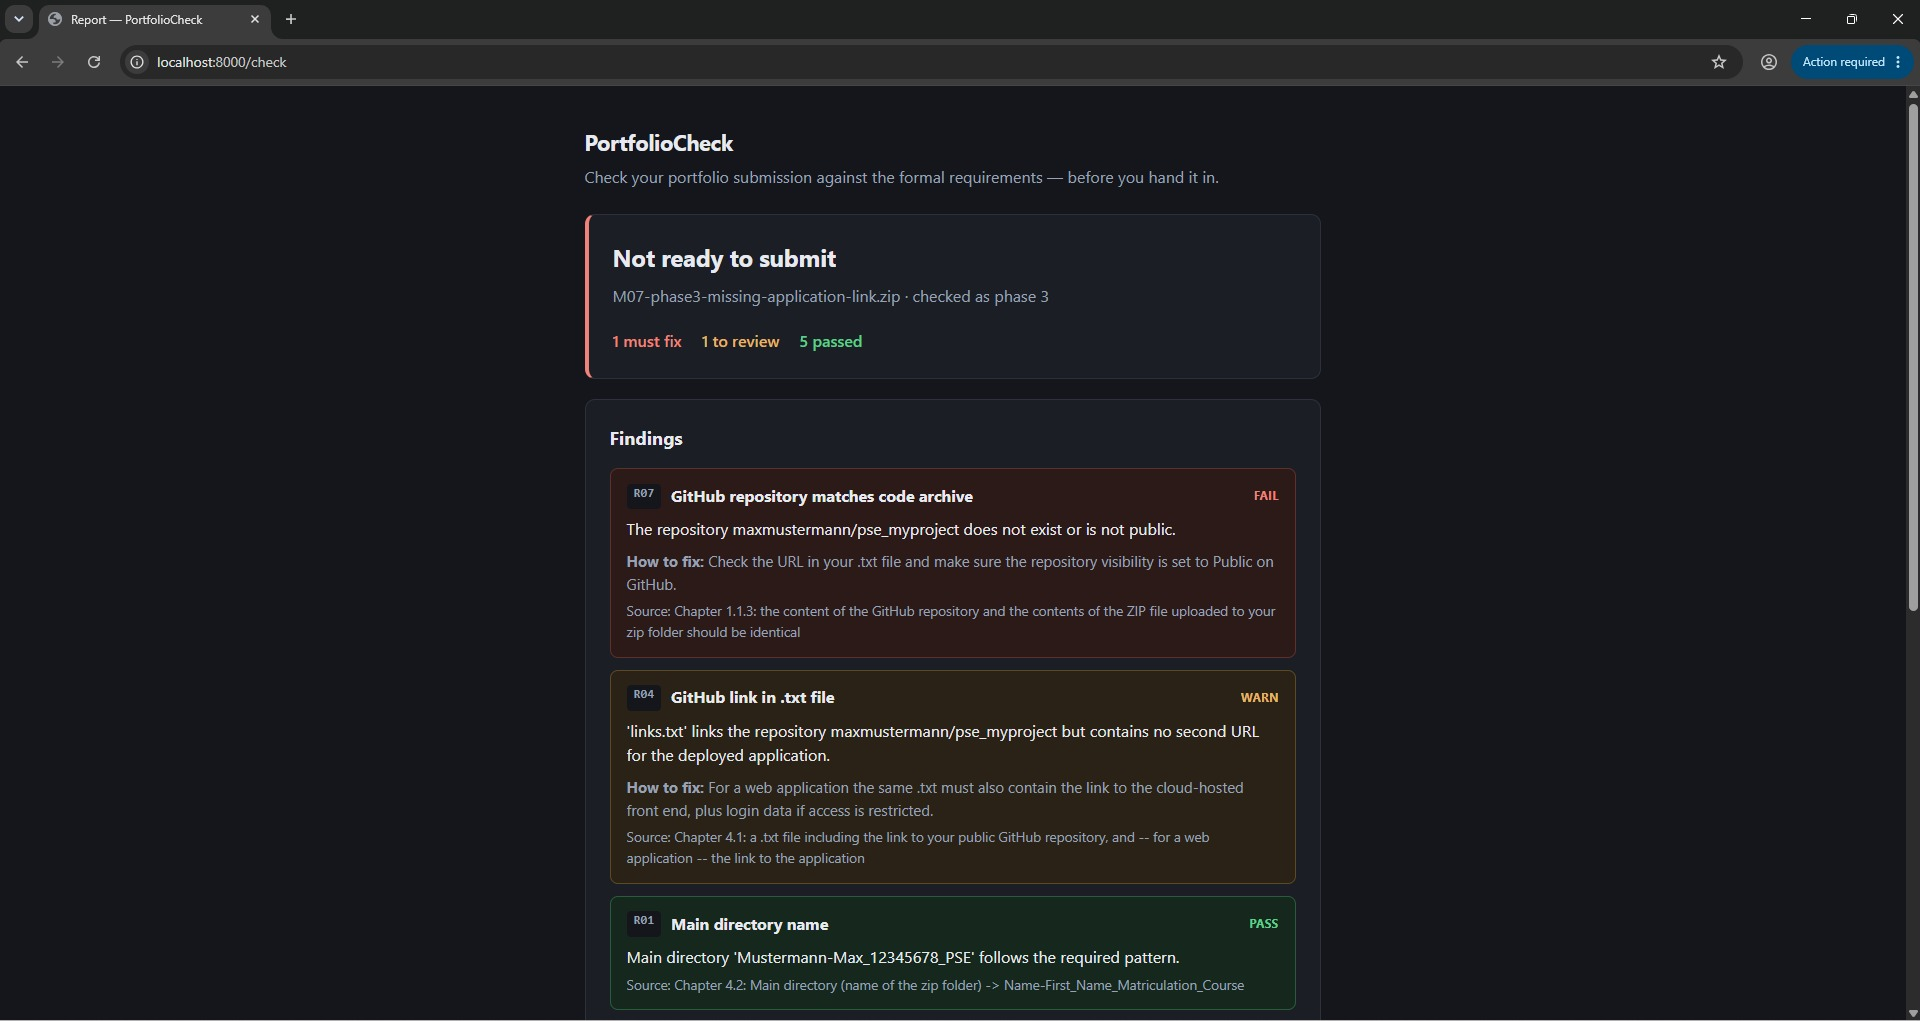
\includegraphics[width=0.97\textwidth]{screenshots/appendix/M07_missing_application_link.jpg}}
\caption{M07, phase 3: links file without application URL --- R04 warns}
\end{figure}

\begin{figure}[H]
\centering
\fbox{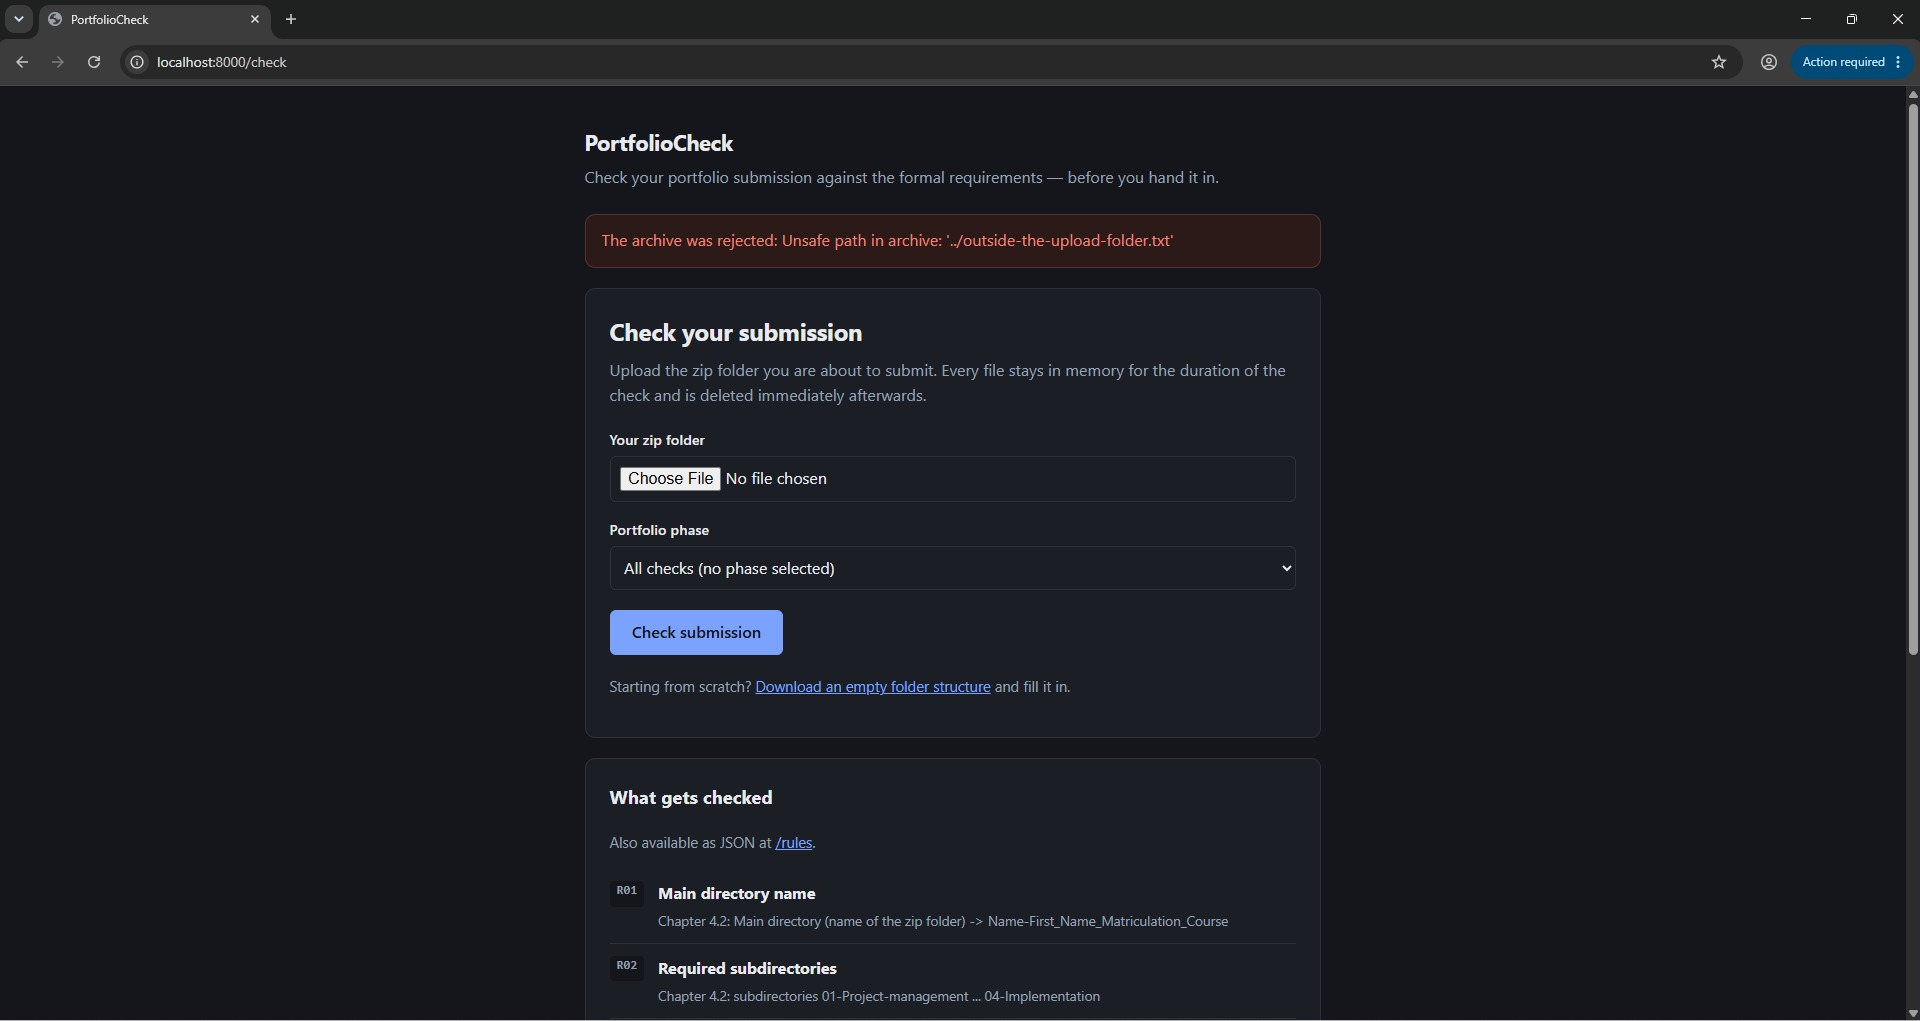
\includegraphics[width=0.97\textwidth]{screenshots/appendix/M08_unsafe_path_traversal.jpg}}
\caption{M08: archive containing a \texttt{../} path --- rejected before extraction}
\end{figure}

\begin{figure}[H]
\centering
\fbox{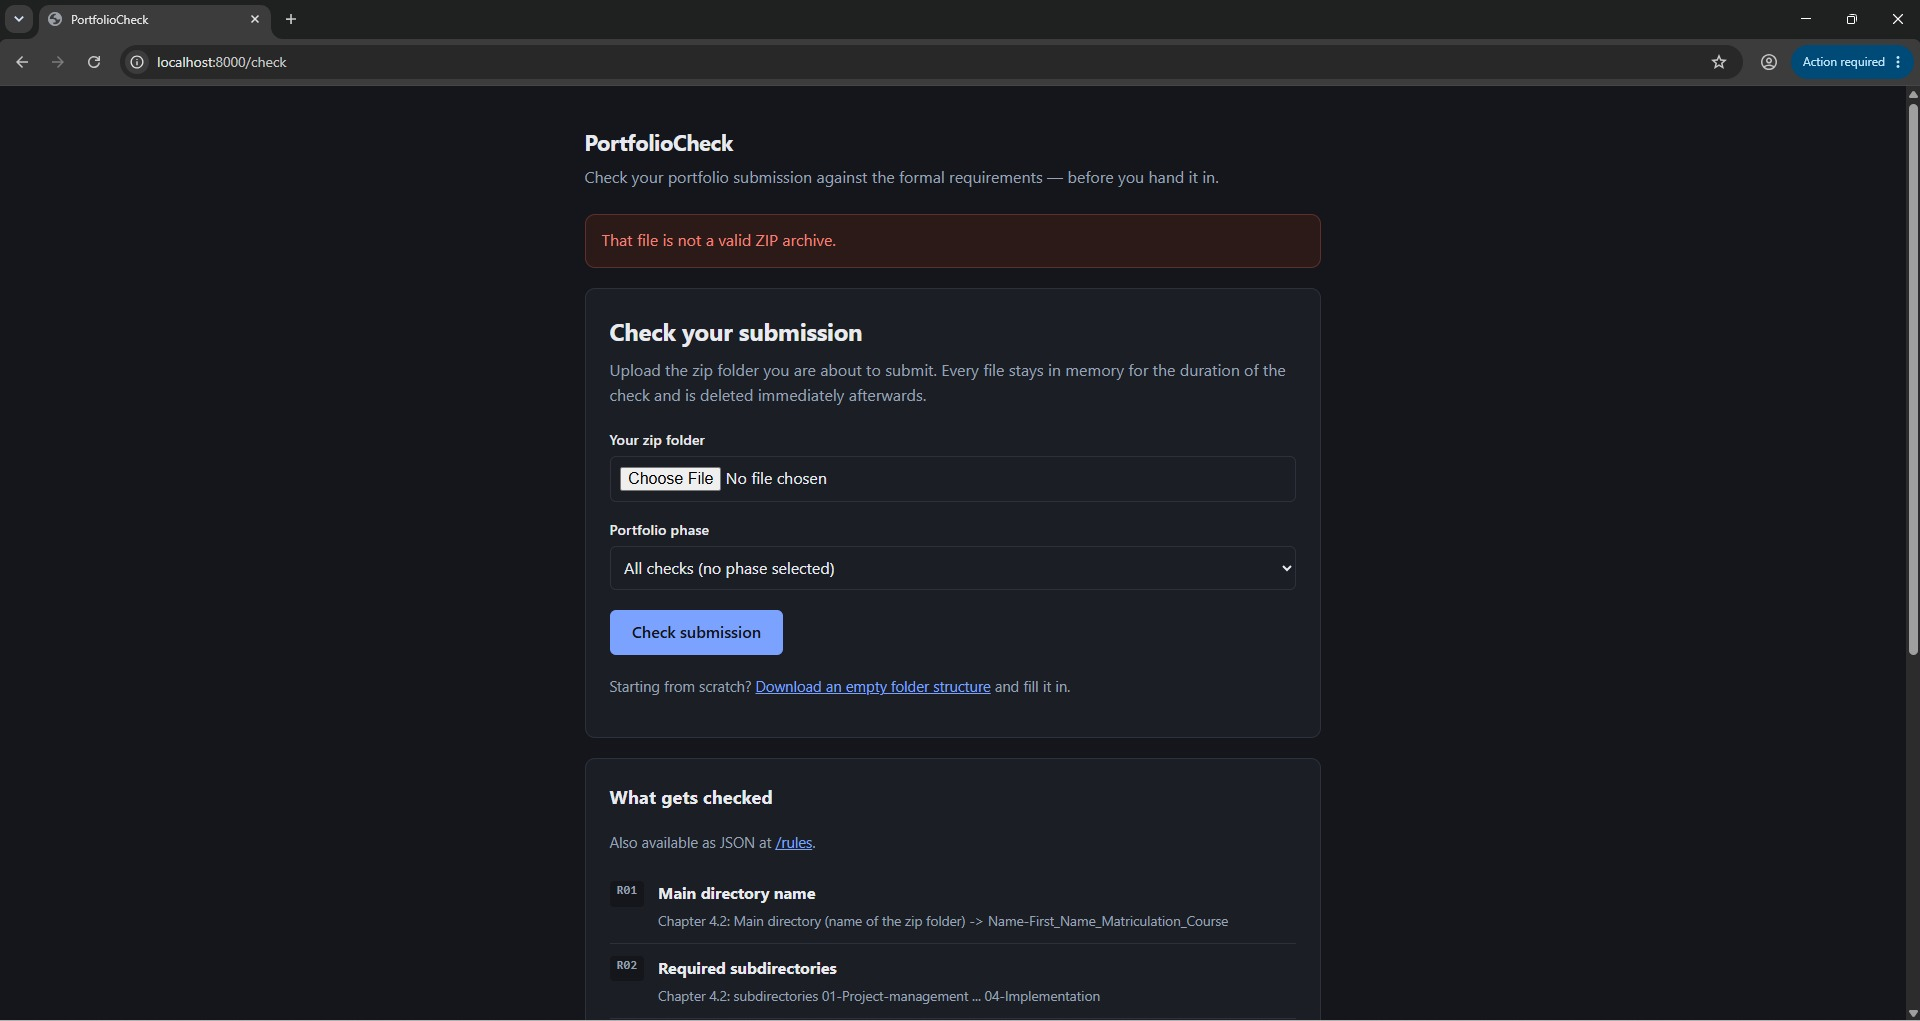
\includegraphics[width=0.97\textwidth]{screenshots/appendix/M09_not_a_zip.jpg}}
\caption{M09: text file renamed to \texttt{.zip} --- rejected as invalid}
\end{figure}

\begin{figure}[H]
\centering
\fbox{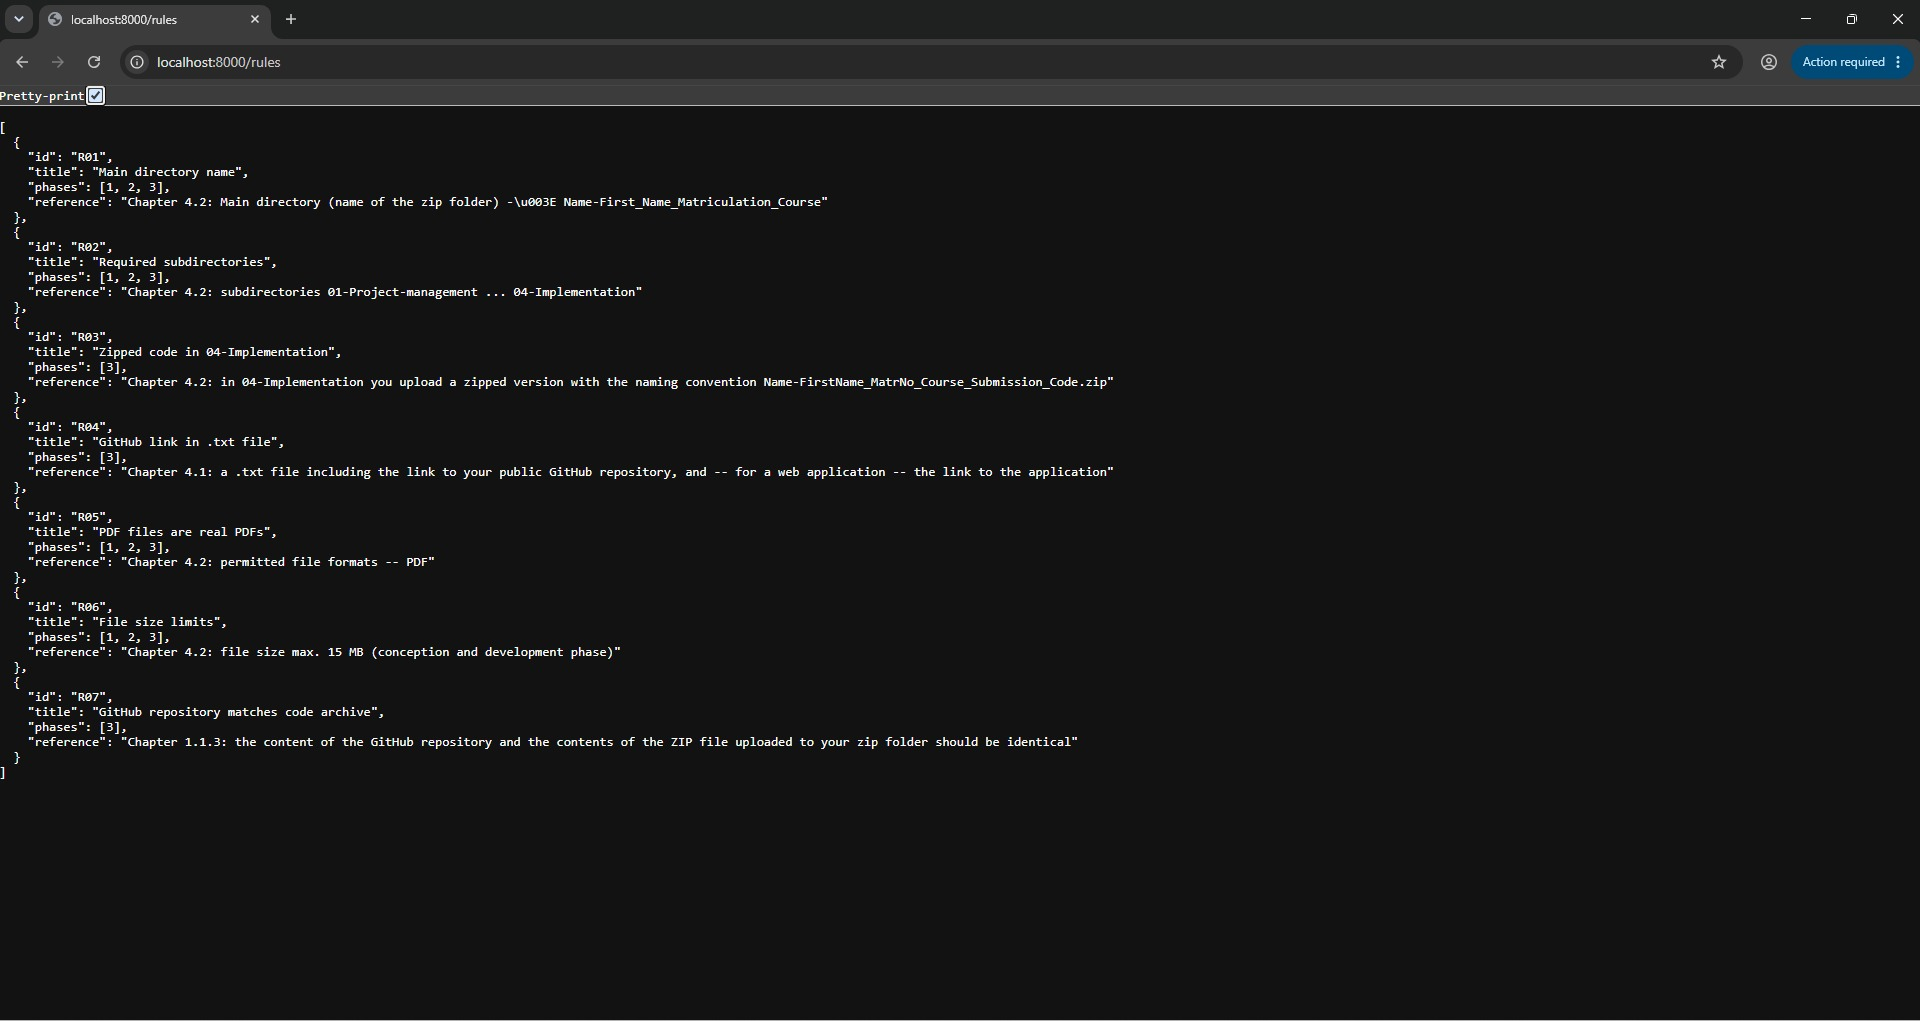
\includegraphics[width=0.97\textwidth]{screenshots/appendix/rules_catalogue_json.jpg}}
\caption{Rule catalogue at \texttt{/rules}: all seven rules with their phases and sources}
\end{figure}

\begin{figure}[H]
\centering
\fbox{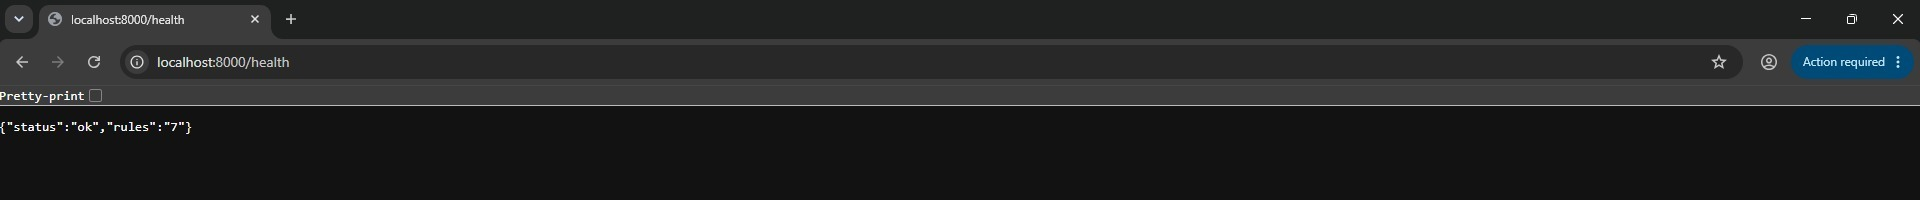
\includegraphics[width=0.97\textwidth]{screenshots/appendix/health_endpoint.jpg}}
\caption{Health endpoint at \texttt{/health}, used by the cloud host to monitor the service}
\end{figure}

\begin{figure}[H]
\centering
\screenshot{screenshots/render_live.jpg}{0.97\textwidth}{Render dashboard showing the service as Live}
\caption{The application deployed on Render}
\label{fig:render}
\end{figure}

\begin{figure}[H]
\centering
\screenshot{screenshots/test_run.jpg}{0.52\textwidth}{pytest run}
\caption{Automated test run: all 73 tests pass}
\label{fig:pytest}
\end{figure}

\end{document}
